\documentclass[onecolumn, 12pt]{book}

\usepackage[latin1]{inputenc}   
%\usepackage[francais]{babel}     
\usepackage{algorithm}
\usepackage{algorithmic} 

\usepackage{layout}    
\usepackage[top=2cm, bottom=2cm, left=2cm, right=2cm]{geometry} 
\usepackage{setspace}
\usepackage{soul}
\usepackage{color} 
\usepackage{verbatim}
\usepackage{moreverb}
\usepackage{listings}
\usepackage{url}
\usepackage{graphicx}
\usepackage[outdir=/home/willy/Documents/latexDoc/redaction/fusion_fichiers/images_fusionChapitres/]{epstopdf}
\usepackage{caption}
\usepackage{setspace}
\usepackage{amsmath, amsthm, amssymb}
\usepackage{amsfonts}
\usepackage{placeins}
 
\title{chapitre3: D\'ecouverte de topologie par les corr\'elations}
\author{Wilfried Ehounou}
\date{\oldstylenums{\today}} 

\newtheorem{definition}{D\'efinition}
\newtheorem{property}{Propri\'et\'e}
\newtheorem{theorem}{Th\'eor\`eme}
\newtheorem{claim}[theorem]{Claim}
\newtheorem{proposition}{Proposition}
\newtheorem{lemma}{Lemme}
\newtheorem{corollary}{Corollaire}
\newtheorem{conjecture}{Conjecture}
\newtheorem{observation}{Observation}
\newtheorem{example}{Exemple}
\newtheorem{remark}{Remarque}

%---insert paragraph (use 4) and subparagraph (use 5) to table of contents
%\setcounter{tocdepth}{4} 
%\setcounter{secnumdepth}{4}

%---- path figures ----
\graphicspath{{/home/willy/Documents/courbePython/courbeDegreCoutMinAleatoire_11_09_2017/}
{/home/willy/Documents/courbePython/courbeDegreCoutMinAleatoire_11_10_2017/}
{/home/willy/Documents/courbePython/courbeDegreCoutMinAleatoire_11_09_2017/comparaison_MethodesCorrection_fctDeCout_permut_aleatoire_coutMin_degreMin/}
{/home/willy/Documents/latexDoc/redactionThese/fusion_fichiers/images_fusionChapitres/}}
 
 \newcommand{\overbar}[1]{\mkern 1.5mu\overline{\mkern-1.5mu#1\mkern-1.5mu}\mkern 1.5mu}
 %---- add name algorithm 
 \makeatletter
\renewcommand{\ALG@name}{Algorithme}
\makeatother

\begin{document}
\maketitle
%\tableofcontents
%--------------------------------------------------------------------
%------- formulation du probleme ---------------------
%--------------------------------------------------------------------
\section{Formulation du Probl\`eme}

	%------- introduction_matrice_correlation ---------
	Consid\'erons un r\'eseau \'electrique modelis\'e par un {\em DAG} $G_F$ et une matrice de corr\'elation $\mu_C$ dans laquelle chaque ligne ou colonne est associ\'ee \`a un arc du graphe $G_F$.
Chaque case $\mu_C[i,j]$ contient une valeur comprise entre $0$ et $1$ qui est la corr\'elation entre les arcs $i$ et $j$. 
Id\'ealement, une corr\'elation proche de $1$ indique que les arcs partagent un sommet peu importe l'extremit\'e (finale ou initial) et dans le cas contraire, elle est proche de $0$. 
Toutefois, il existe des erreurs de mesures sur les arcs entrainant des erreurs de corr\'elation dans la matrice $\mu_C$. Une erreur de corr\'elation est une valeur proche de $1$ (respectivement de $0$) alors que les arcs n'ont aucun sommet en commun (respectivement partage un sommet).
\newline
En choisissant un seuil ${\cal S} = [0,1]$, nous consid\'erons  la matrice $M$ de m\^eme dimension que $\mu_C$ telle que $M[i,j] = 1$ ssi $\mu_C[i,j] \ge {\cal S}$ sinon $M[i,j] = 0$.
\newline
Soit $G_M = (V, E)$ un graphe non orient\'e dont $M$ est la matrice d'adjacence obtenue par application du seuil $\cal S$ \`a $\mu_C$. 
Si   $\mu_C$ ne contient aucune erreur de corr\'elation et que $\cal S$ est bien choisi alors $G_M$ est le line-graphe du $G_F$. Notre probl\`eme est alors de corriger ces erreurs  permettant d'obtenir le line-graphe le plus proche du line-graphe du $G_F$.
\newline
Dans ce chapitre, nous expliquerons l'utilit\'e des line-graphes dans la reconstruction de topologie. Ensuite nous d\'efinirons le probl\`eme et les algorithmes de r\'esolution de celui-ci. Enfin nous \'evaluons nos algorithmes dans les conditions extr\^emes ($M$ ne contient que des erreurs de corr\'elation).

	%------- caracteristiques_linegraphes ----------------
	\subsection{Caracteristiques d'un line-graphe}
		Dans la litt\'erature, le {\em line-graphe} est d\'esign\'e par le {\em graphe adjoint} ou {\em linegraph}. 

\begin{definition}
Soit $G=(V,A)$ un DAG. 
Le line-graphe de $G$ est un graphe non-orient\'e $L(G) = (V',E)$ o\`u $V'=A$ et une paire $[a,a']$ de sommets de $L(G)$ est une ar\^ete ssi $a$ et $a'$ ont une extremit\'e commun (peu importe l'extremit\'e initial ou finale comme dans la figure \ref{typeSommetsEnCommun}) dans $G$.
\end{definition}

\begin{figure}[htb!]\vspace{-0.5em}
	\centering
	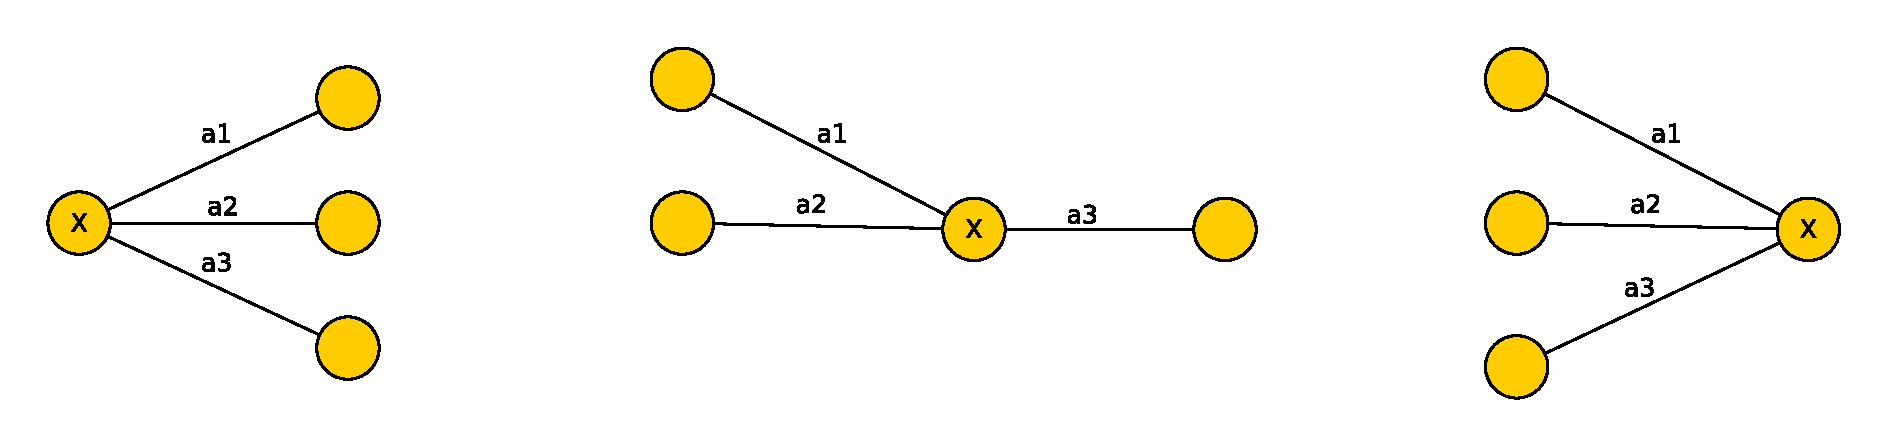
\includegraphics[scale=0.50]{typeSommetsEnCommun.eps}\vspace{-0.5em}
	\caption{ Sommet $X$ partag\'e entre les ar\^etes. De la gauche vers la droite : sommet entrant, \`a droite sommet interm\'ediaire et sommet sortant }\vspace{-0.5em}
	\label{typeSommetsEnCommun}
\end{figure}

Avec $G$ ayant $n$ sommets et $m$ arcs, le graphe $L(G)$ a $m$ sommets et $E$ ar\^etes dont 
$$ E = \sum_{i=1 }^{n} d_i(d_i -1)/2$$, 
$d_i$ \'etant le degr\'e de chaque sommet $i$ de $G$.
Le graphe $G$ est  appel\'e le {\em graphe racine} de $L(G)$. 
Un exemple de graphe racine et son line graphe est present\'e dans la figure \ref{rootGrapheLineGrapheExemple}

\begin{figure}[htb!]\vspace{-0.5em}
	\centering
	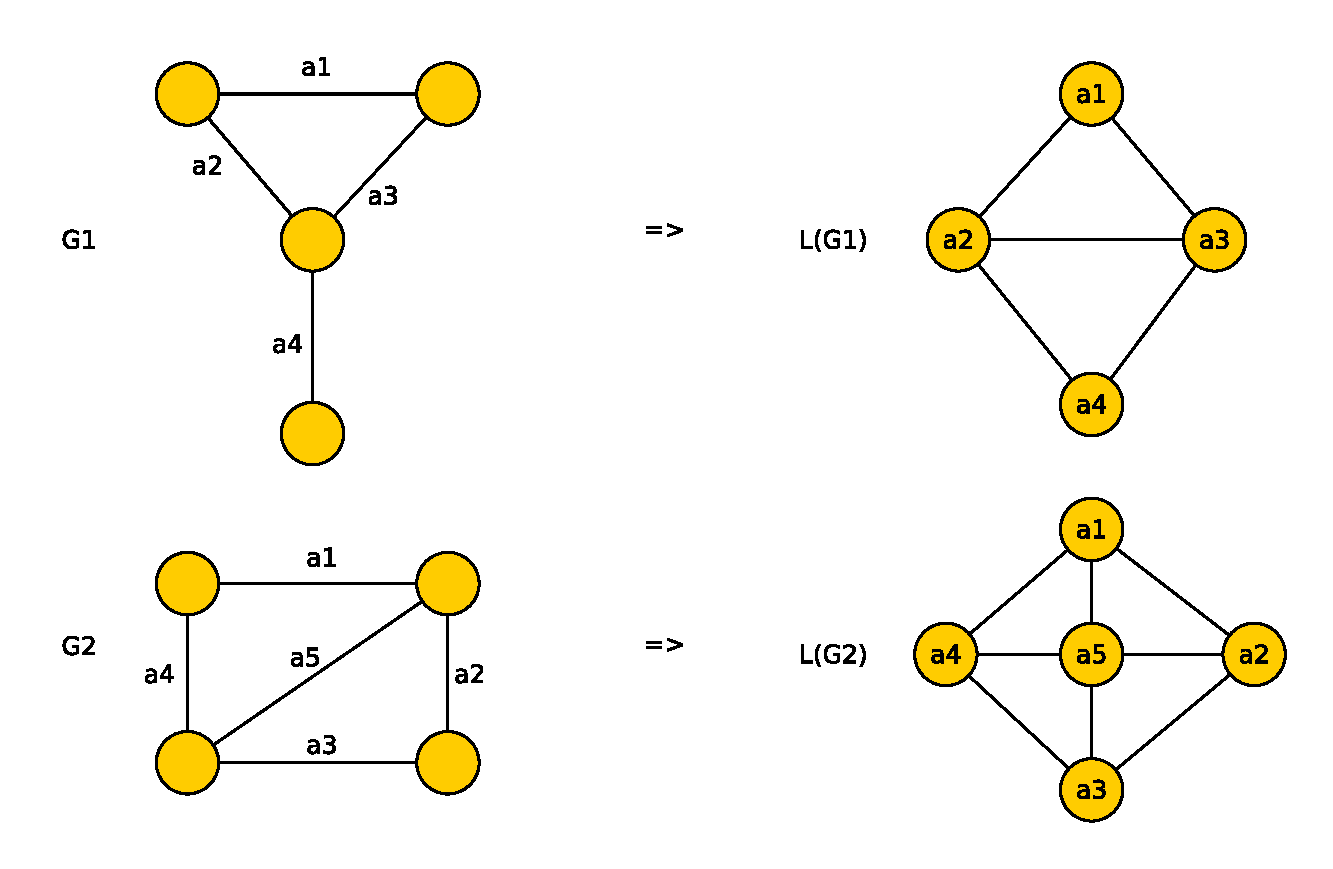
\includegraphics[scale=0.50]{rootGrapheLineGrapheExemple.eps}\vspace{-0.5em}
	\caption{ Le graphe racine $G$ et son line graphe L(G) }\vspace{-0.5em}
	\label{rootGrapheLineGrapheExemple}
\end{figure}

La notion de line-graphe a \'et\'e introduite par {\em Whitney} \cite{isomorphismeLineGraphe} \`a partir de l'isomorphisme d'ar\^etes. Il montra que l'isomorphisme des ar\^etes implique l'isomorphisme de graphes connexes \`a condition que ces graphes connexes soient diff\'erent de $K_{1,3}$(graphe \'etoile) et $K_3$(graphe triangle).
\begin{proposition}
Le graphe \'etoile $K_{1,3}$ n'est pas un {\em line graphe}.
\end{proposition}
\begin{proof}
Supposons que $K_{1,3}$ est le line graphe de $H$ ($K_{1,3} = L(H)$). 
Alors $H$ est un graphe connexe de quatre ar\^etes.
Tous les graphes connexes de quatres ar\^etes sont repr\'esent\'es dans la figure  \ref{graphesRacinesDeQuatresAretes}. 
Comme $L(C_4) = C_4$  et $L(K_{1,3} + e) = K_4 + e$ (voir figure \ref{rootGrapheLineGrapheExemple}), $L(H)$ ne peut \^etre que l'un des trois arbres $P_4$, $K_{3,2}$ et $K_{1,4}$.
Ce qui est contraire \`a notre hypoth\`ese de d\'epart ($K_{1,3} = L(H)$).
\end{proof}

\begin{figure}[htb!]\vspace{-0.5em}
	\centering
	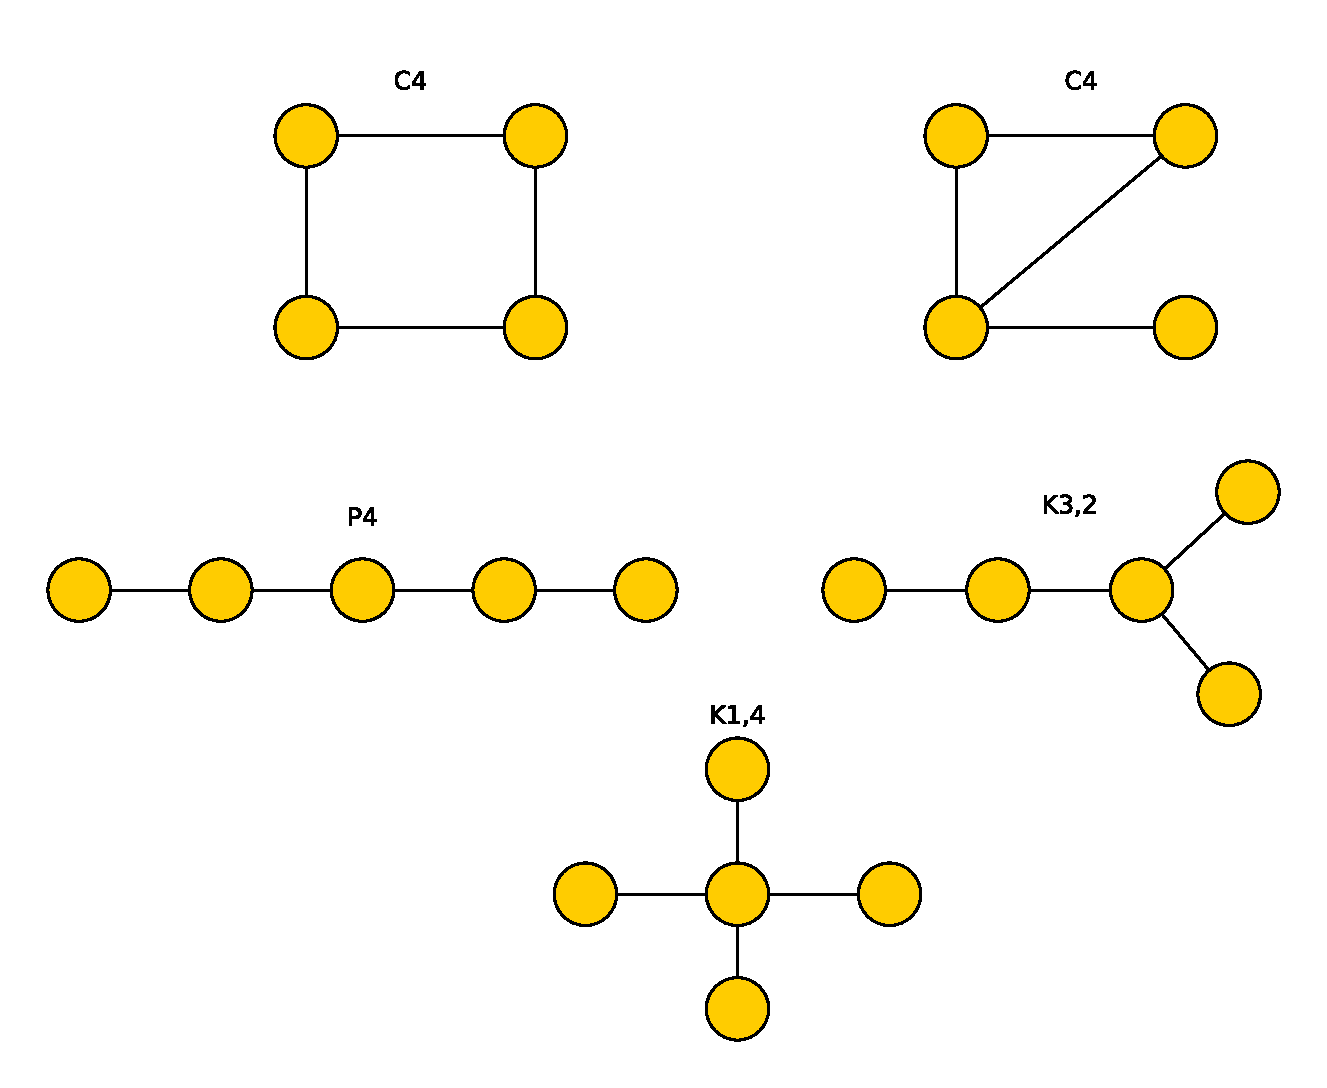
\includegraphics[scale=0.50]{graphesRacinesDeQuatresAretes.eps}\vspace{-0.5em}
	\caption{ Les graphes racines possibles de $K_{1,3}$ de quatres ar\^etes   }\vspace{-0.5em}
	\label{graphesRacinesDeQuatresAretes}
\end{figure}

Le graphe \'etoile ($K_{1,3}$) joue un r\^ole important dans la caracterisation des line-graphes.
La premi\`ere propri\'et\'e, provient de {\em Krausz} \cite{krausz1943demonstration} et est relatif au partitionnement du line-graphe en sous-graphes. La seconde, edit\'e par {\em van Rooij and wilf} \cite{ROOIJetWILF1965interchange}, d\'ecrit la structure de base d'un graphe pour \^etre un line-graphe. Et enfin {\em Beineke\cite{beineke1968derived} et Hemminger}   affichent les neufs sous-graphes ne pouvant pas avoir de line graphes. 
\begin{theorem}
\label{caracteristiquesLinegraphes}
Soit $H$ un line-graphe. Les affirmations suivantes sont \'equivalentes.
\begin{itemize}
	\item les ar\^etes de $H$ peuvent \^etre partition\'ees en sous graphes complets tel que aucun sommet est contenu dans plus de deux sous-graphes. Ces sous graphes complets sont des cliques.
	\item $H$ ne contient pas $K_{1,3}$ comme sous-graphe et si deux triangles ont une ar\^ete commune alors le sous graphe induit est $K_4$.
	\item Aucun des neufs sous-graphes de la figure \ref{neufSousGraphesInterditDesLineGraphes} ne peut \^etre un sous graphe d'un line graphe $G$.
\end{itemize}
\end{theorem}

\begin{figure}[htb!]\vspace{-0.5em}
	\centering
	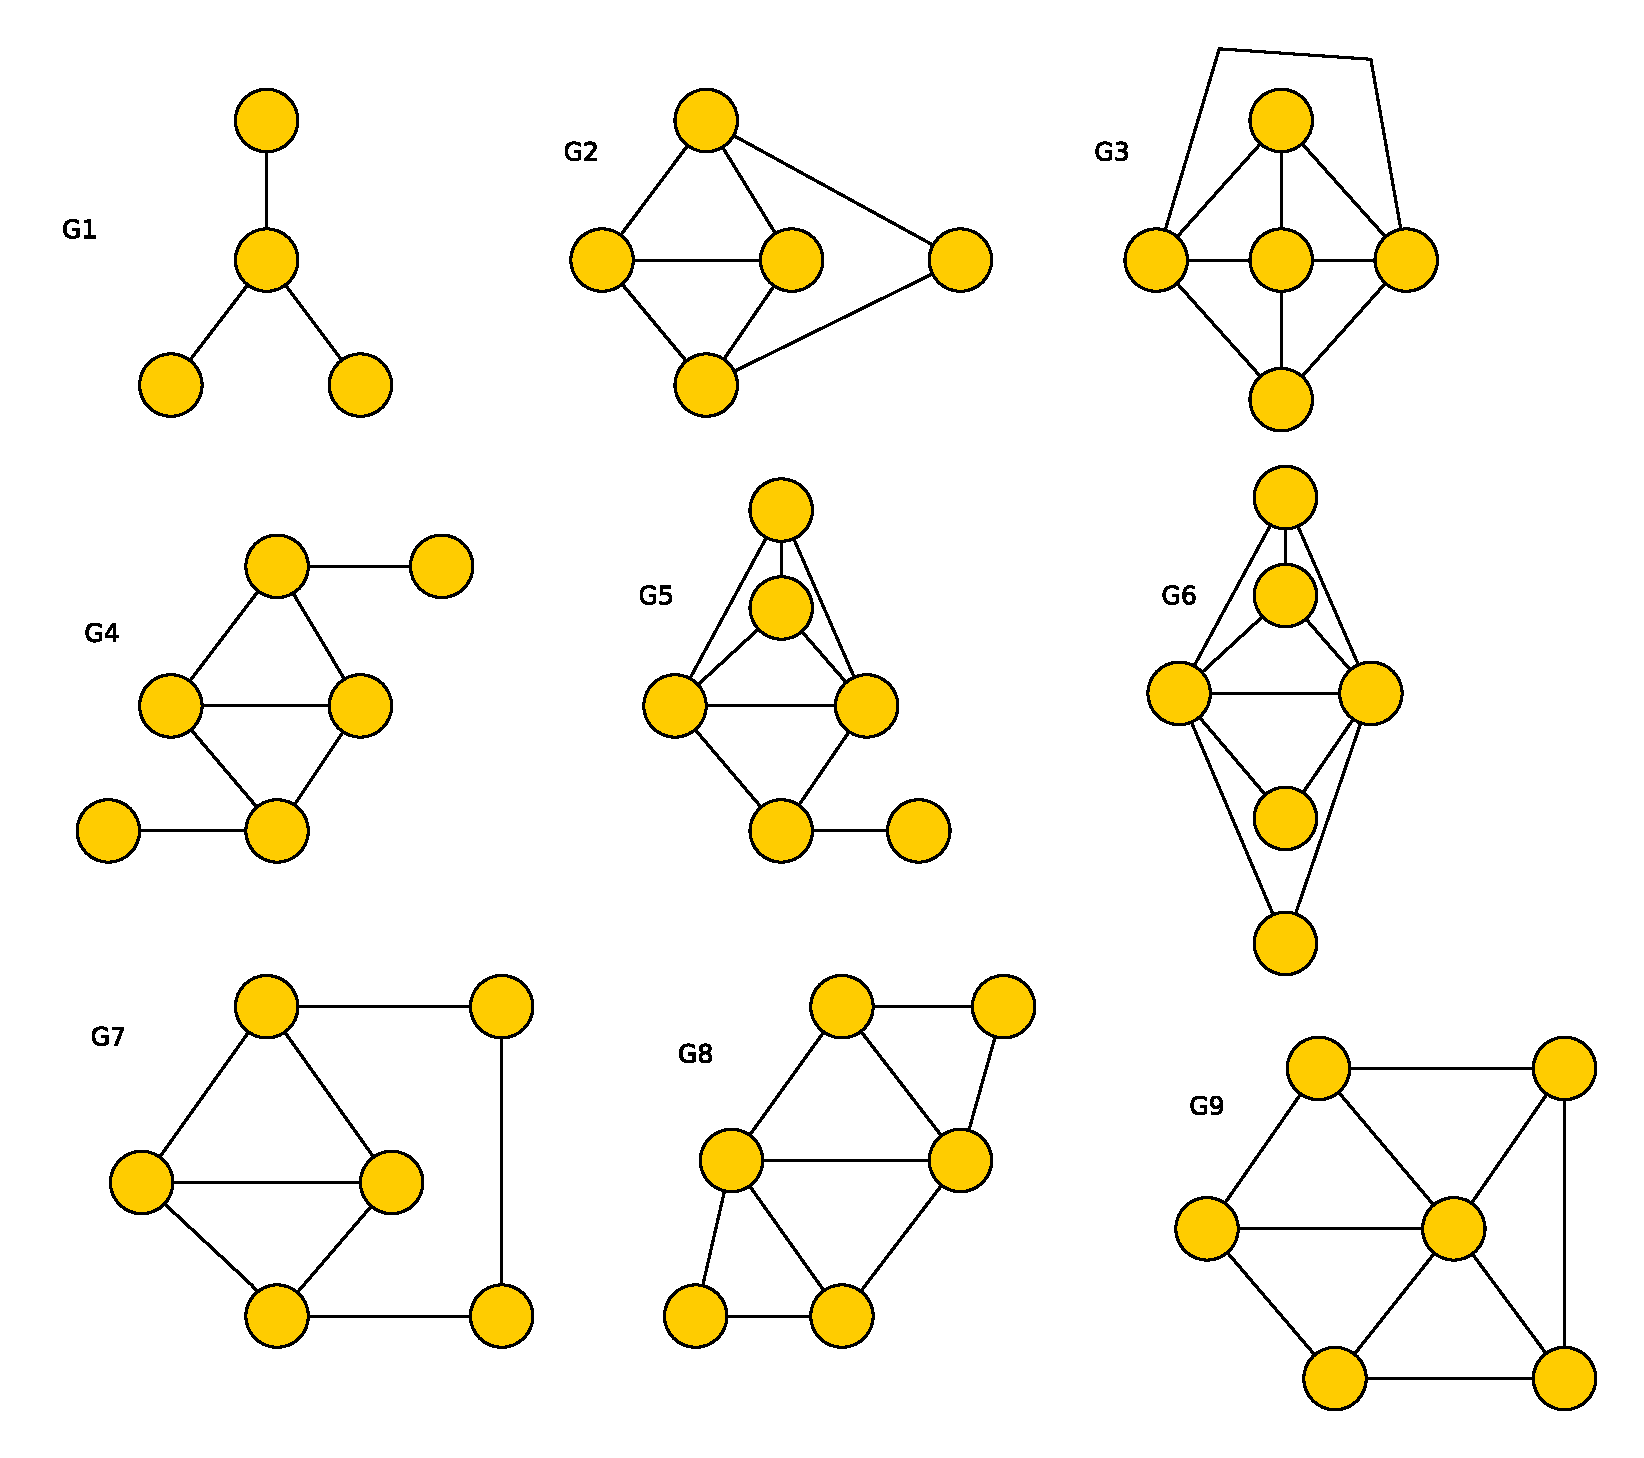
\includegraphics[scale=0.50]{neufSousGraphesInterditDesLineGraphes.eps}\vspace{-0.5em}
	\caption{ Line graphes et sous graphes interdits }\vspace{-0.5em}
	\label{neufSousGraphesInterditDesLineGraphes}
\end{figure}

\begin{proof}
Voir theor\`eme 8.4, chapitre 8 \cite{lineGraphe}.
\end{proof}


	%------- proprietes_linegraphes -------------------------
	\subsection{Propri\'et\'es d'un line-graphe}
		Nous souhaitons non seulement v\'erifier if $G_M$ est un line-graphe mais aussi trouver le graphe racine de $G_M$, un DAG modelis\'e par un r\'eseau \'electrique sans ambiguit\'e.
\newline 
\begin{definition}
	Le graphe $G_M$ est un graphe de corr\'elation ssi il est le line graphe d'un DAG.
\end{definition}
D'apr\`es le theor\`eme \ref{caracteristiquesLinegraphes}, L'ensemble des cliques $\cal C$ est dit une {\bf couverture de corr\'elation} de $G_M$.

\begin{definition}
Une ambigu\"{i}t\'e est un graphe isomorphe \`a l'un des graphes de la figure \ref{configurationAmbiguite}. Le sommet $X$ est appel\'e le {\bf point d'ambiguit\'e}.
\end{definition}

\begin{figure}[htb!]\vspace{-0.5em}
	\centering
	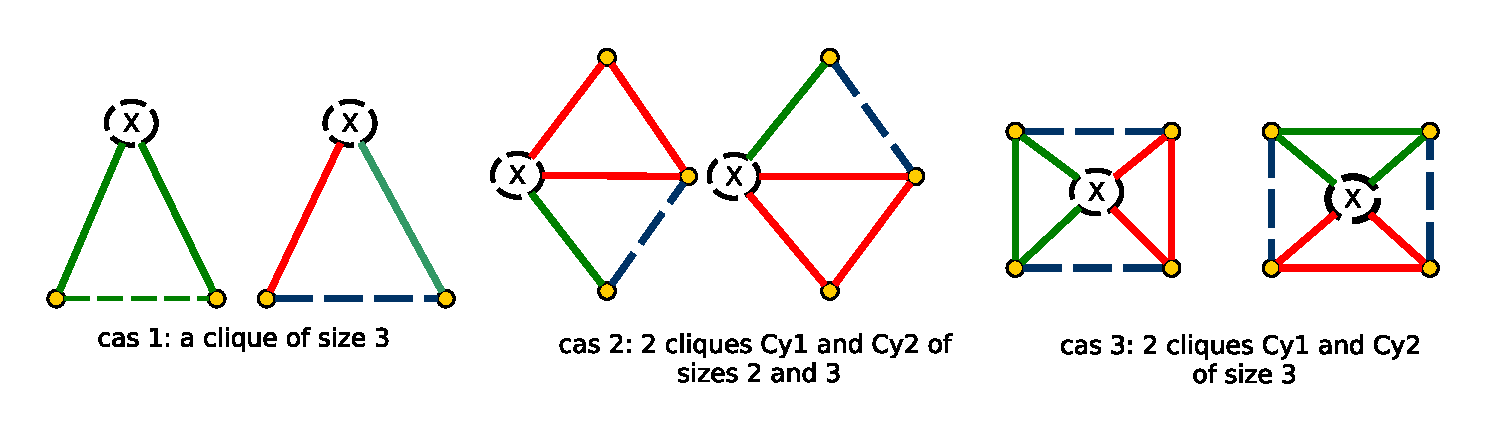
\includegraphics[scale=0.70]{configurationAmbiguite.eps}\vspace{-0.5em}
	\caption{ Configurations possibles d'une ambiguit\'e au sommet X }\vspace{-0.5em}
	\label{configurationAmbiguite}
\end{figure}

\begin{lemma}
	Si un graphe de corr\'elation $G_M$ admet deux couvertures de corr\'elation, alors il existe au moins un sommet $u$ de $G_C$ tel que $G_{C}[\{u\} \cup \Gamma_{G_C}(u)]$ est une ambiguit\'e dont $u$ est le point.
\end{lemma}
	
\begin{proof} 
	Consid\'erons deux line-couvertures $C$ et $C'$ de $G_C$. 
	Il existe au moins un sommet $v \in G_C[V]$ qui n'est pas couvert par la (ou les) m\^eme(s) clique(s) dans $C$ et $C'$.
	Soient deux cliques $c_1$ et $c_2$ (potentiellement vide) partitionant $\{v\} \cup \Gamma_{G_C}(v)$ dans $\cal C$.
	Consid\'erons deux autres cliques $c_3$ et $c_4$ diff\'erentes de $c_1$ et $c_2$ partitionant \'egalement $\{v\} \cup \Gamma_{G_C}(v)$ dans $\cal C$. \newline
	Notons $c_{i,j}$ l'intersection de $c_{i}$ et $c_j$ pour tout $i \in \{1,2\}$ et $j \in \{3,4\}$. 
	Chaque sommet $w \in c_{i,j}$ est couvert par au plus deux cliques de $G$ dans $\cal C$, dont la clique $c_i$.
	Puisque $c_j$ est une clique alors ce sommet $w$ est voisin de tous les sommets de  $c_{i',j}$, pour $i' \ne i$.
	Les ar\^etes entre ces sommets sont dans $c'_i$, donc chaque ar\^ete $[w,z]$ pour tout sommet  $z \in c_{i',j}$ forme une clique correspondant dans le r\'eseau de flots.
	Ainsi, le cardinal de chaque ensemble  $c_{i,j}$ est \'egal \`a $1$.\newline
	Appelons $v_{i,j}$ le seul sommet pr\'esent dans $c_{i,j}$. 
	Il est possible d'avoir $v_{1,3} = v_{1,4}$ ou $v_{2,3} = v_{2,4}$.
	Si les deux \'egalit\'es sont v\'erifi\'ees, le sommet $v$ est alors couvert non pas par deux cliques mais par une seule de cardinalit\'e $3$.
	Ainsi, les seuls cas possibles sont alors r\'esum\'es par la figure  \ref{graphe2Couverture}.
	Le sommet $v$ est bien le point d'une ambigu\"{i}t\'e isomorphe \`a $G_C[\{u\} \cup \Gamma_{G_C}(u)]$.
\end{proof}

Nous d\'eduisons le corollaire suivant :
\begin{corollary}
Si un graphe de corr\'elation admet deux couvertures de corr\'elation, alors il est isomorphe \`a l'un des graphes de la figure  \ref{graphe2Couverture}.
\end{corollary}

\begin{figure}[htb!] \vspace{-0.5em}
\centering
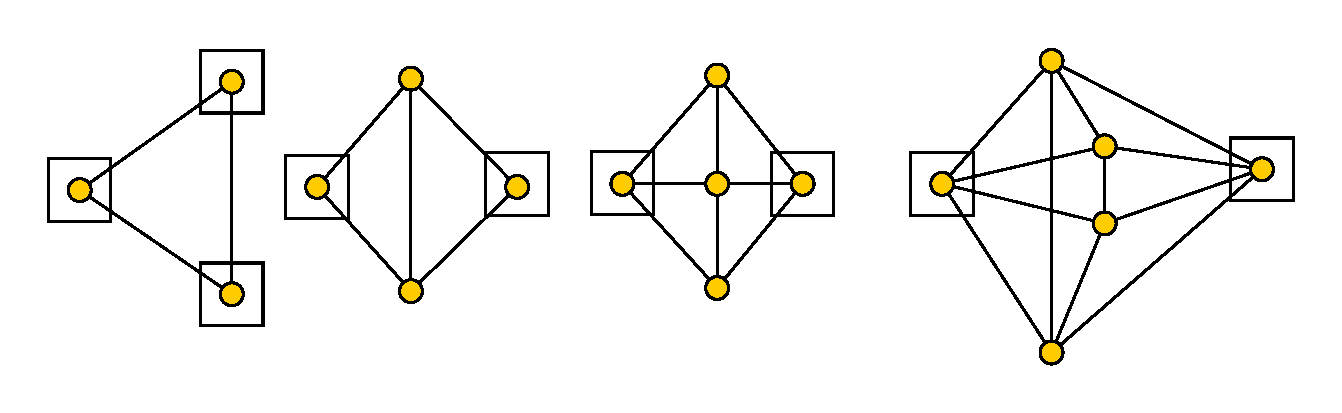
\includegraphics[scale=0.75]{graphe2Couverture.eps}
\caption{ Graphes possibles avec deux couvertures avec les points d'ambigu\"{i}t\'es }
\label{graphe2Couverture} 
\end{figure}
En Effet, si $G_M[\{u\} \cup \Gamma_{G_M}(u)]$ est une ambigu\"{i}t\'e, chaque ar\^ete, qui n'est pas li\'ee au point d'ambigu\"{i}t\'e, doit \^etre une ar\^ete d'une et une seule autre ambigu\"{i}t\'e de $G_M$. Et chaque sommet d'une ambigu\"{i}t\'e, qui n'est pas un point d'ambigu\"{i}t\'e, doit appartenir \`a une et une seule autre ambigu\"{i}t\'e de $G_M$ dont il n'est pas non  plus le point d'ambigu\"{i}t\'e.
De plus, chaque ar\^ete, n'\'etant pas couvert par les deux configurations de cliques possibles dans une ambigu\"{i}t\'e (les ar\^etes en pointill\'ees dans la figure \ref{graphe2Couverture}), doivent \^etre dans la m\^eme situation dans une autre ambigu\"{i}t\'e \`a laquelle elles appartiennent.
Ces contraintes font que si un graphe contient une ambigu\"{i}t\'e induite, alors il ne peut \^etre que dans un cas de la figure  \ref{graphe2Couverture}.

\begin{definition}
Soit $G$ un graphe et $u$ un sommet de $G$. Une partition de $\Gamma_G(v)$ en deux cliques $C_{u1}, C_{u2}$ est {\bf coh\'erente } ssi chaque sommet $v$ de $C_{u1}$ (resp $C_{u2}$) a au plus un voisin dans $C_{u2}$  (resp $C_{u1}$).
\end{definition}
Le r\'esultat suivant est un corollaire direct de la preuve du lemme \ref{lemmaCoherente}
\begin{lemma}
\label{lemmaCoherente}
Soit $G_M$ un line graphe, $u$ un sommet de $G_M$ et une partition coh\'erente de ${u} \cup \Gamma_{G_M}(v)$ en deux cliques  $C_{u1}, C_{u2}$. 
Si l'une de ces deux cliques est de cardinal sup\'erieur ou \'egal \`a $4$, alors cette partition coh\'erente est unique.
\end{lemma}

\'Etant donn\'e une partition coh\'erente $C_{u1}, C_{u2}$ pour un sommet $u$ de $G_M$, la fiabilit\'e de cette coh\'erence est
$$F(C_{u1}, C_{u2}) = \min\limits_{[x,y] \in E(C_{u1}) \cup E(C_{u2})}  \mu_{C}([x,y])$$


Une {\bf line-couverture} d'un graphe non orient\'e connexe $G_C$ est un ensemble de cliques maximales de $G_M$ telles que chaque sommet de $G_C$ appartient \`a une ou deux de ces cliques et que chaque ar\^ete de $G_C$ soit couverte par exactement une de ces cliques.
s'il existe une line-couverture de $G_M$ alors nous supposons que $G_M$ est le v\'eritable  line-graphe du DAG $G$ du r\'eseau \'electrique.
Dans le cas $G_M$ n'est pas un line-graphe alors nous d\'eterminons le line-graphe $G'$ avec le m\^eme ensemble de sommets que $G_M$ minimisant la distance avec $G_M$ d\'efinie dans la partie suivante.


	%------- probleme -----------------------------------------------
	\subsection{Probl\`eme}
		\begin{definition}
Soient $G$ et $G'$ deux graphes ayant le m\^eme ensemble  de sommets.
%La distance en $G$ et $G'$ est la distance de Hamming not\'ee $DH(G,G')$ entre leurs deux matrices d'adjacente, c'est-\`a-dire le nombre d'\'el\'ements ayant une valeur diff\'erente dans chacune des deux matrices.
La distance de Hamming entre $G$ et $G'$ not\'ee $DH(G,G')$ est le nombre d'\'el\'ements ayant une valeur diff\'erente dans chacune des deux matrices d'adjacence.
\end{definition}
Une distance de Hamming \'egale \`a $k$ $(k \in \mathbb{N})$ signifie qu'il existe $k$ ar\^etes diff\'erentes entre  les graphes $G$ et $G'$.

\begin{definition}
On appelle distance-line de $G$, not\'ee $DL(G)$, la plus petite distance de Hamming entre $G$ et $G'$, $G'$ \'etant le line graphe d'un DAG ayant le m\^eme ensemble de sommets que $G$.
\end{definition}

Nous consid\'erons le probl\`eme suivant. \newline
{\bf Probl\`eme} Proxi-Line \newline
{\bf Donn\'ees} : Un graphe $G=(V,E)$, un entier $k$. \newline
{\bf Question} : $DL(G) \le k$ ? \newline

\begin{conjecture}
Proxi-Line est NP-complet.
\end{conjecture}

La preuve de la conjecture est en annexe 1.

%-----------------------------------------------------------------------------------------------------------
%------- algorithme de decouverte: couverture et correction ---------------------
%-----------------------------------------------------------------------------------------------------------
\section{Algorithmes de d\'ecouverte de topologie}

	Il a \'et\'e montr\'e qu'un graphe $G_C$ est  un line graphe si et seulement si il admet une line-couverture.
Bas\'ee sur cette id\'ee et sur des sous-graphes exclus, un algorithme lin\'eaire en fonction du nombre d'ar\^etes a \'et\'e propos\'e pour v\'erifier  si un graphe est un line graphe et si oui en fournir la line-couverture.
Cette algorithme est {\bf l'algorithme de couverture}.
	\subsection{Algorithme de couverture}
		L'algorithme de couverture est une am\'elioration de  celui de Lehot \cite{decompositionEnCliquesParArcs}.
En effet, l'algorithme de Lehot se subdivise en deux parties : 
La premi\`ere partie consiste \`a nommer des sommets appartenant \'a une m\^eme clique et la seconde partie \`a comparer, s'il existe, le line graphe propos\'e avec celui du graphe racine. 
Concernant l'identification, il distingue 5 categories de sommets:
\begin{itemize}
\item les sommets ``well-defined" : des sommets du graphe racine $G$ dont leur clique correspondante dans $L(G)$ a \'et\'e trouv\'ee et identifi\'ee.
\item les sommets ``half-named" : des sommets de $L(G)$ dont un sommet de leur ar\^ete dans $G$ a d\'ej\`a \'et\'e ``well-defined".
\item les sommets ``fully-named" : des ar\^etes de $G$ dont leurs sommets dans $L(G)$ sont "well-defined".
\item les sommets ``basics" : sommets adjacents dans $L(G)$. Not\'e $2-3$, chaque chiffre est un sommet dans $G$.
\item les sommets ``cross" : sommets adjacents aux sommets ``basics" appartenant \`a deux cliques.
\end{itemize}
Le but de cet algorithme est d'identifier les sommets ``cross" parmi les sommets adjacents d'un sommet de $L(G)$ \`a partir des trois cas \cite{decompositionEnCliquesParArcs}. \newline
L'algorithme d\'ebute par la s\'election de deux sommets ``basics" $1-2, 2-3$ et de leur ensemble d'adjacents $X$.
Si $|X| = \emptyset$ alors tous les sommets des cliques sont identifi\'es en ``half-named".
Si $|X| = 1$ alors il existe un sommet $x$ adjacent aux deux sommets ``basics" ($1-2,2-3$) tel que $(x,1-2,2-3)$ forme un triangle ``odd" si $x=2-4$ ou un triangle ``even" si $x=1-3$. Le sommet $x$ devient {\em cross} et est identifi\'e en ``fully named". Les autres sommets $1-2,2-3$ sont identifi\'es en ``half-named".
Dans le cas o\`u  $|X = \{x,y\}|=2$, si $x$ et $y$ sont adjacents alors il n'existe pas de sommets ``cross" sinon ils forment deux triangles avec $1-2,2-3$. Un de ces triangles est ``odd" implique que $x=2-4$ , $y=1-3$ et $y$ est identifi\'e en sommet ``cross".
Enfin pour $|X =\{ a,b,...\}| \ge 3$, si $a$ et $b$ sont adjacents, $b$ est d\'eclar\'e sommet ``cross" sinon c'est le sommet $a$ qui le devient.
La derni\`ere \'etape s\'electionne al\'eatoirement un sommet $u$ ``half-named". Ce sommet est adjacent \`a un sommet $v$ ``fully-named". Si ce sommet $v$ n'est pas d\'ej\`a couvert par une clique, alors il existe un sommet $z$ ``fully-named" qui appartient d\'ej\`a \`a une clique et qui est d\'eclar\'e sommet ``cross" de ces deux pr\'ec\'edents sommets $u$ et $v$. Nous trouvons ces sommets $u$ et $v$ gr\^ace \`a une pile o\`u $u$ et $v$ sont en t\^ete et nous les nommons avec le num\'ero de la clique. 
\`A la fin de cette \'etape, tous les sommets sont nomm\'es ``fully-named" et nous identifions les sommets ``fully-named" adjacents par un nouveau num\'ero de clique.
\newline
Nous comparons le line-graphe propos\'e $H$ et le line-graphe $L(G)$ de $G$, ar\^etes par ar\^etes, et s'il existe une ar\^ete de $H$ n'ayant pas de correspondance dans $L(G)$ alors $L(G)$ n'est pas un line-graphe et l'algorithme ne retourne pas de r\'esultats c'est-\`a-dire aucunes cliques d\'ecouvertes lors du traitement des sommets.
Cet algorithme s'ex\'ecute en $O(N)+E$ avec $N$  le nombre d'ar\^etes dans $G$ et $E$ le nombre d'ar\^etes dans $L(G)$ car le processus d'identification des ar\^etes est en $O(N)$ et la comparaison entre graphes en $E$ \'etapes.
\newline

Notre algorithme de couverture  couvrira autant que possible des sommets du graphe de corr\'elation  $G_M$ par une ou deux cliques et si $G_M$ ne contient aucune erreur de corr\'elation alors il retourne sa line-couverture. Dans le cas contraire, les sommets couverts par plus de deux cliques sont sauvegard\'es dans l'ensemble des sommets \`a corriger $sommets\_1$ et notre algorithme retourne les cliques d\'ecouvertes et l'ensemble $sommets\_1$.

\subsubsection{Description de l'algorithme de couverture}
Soit le graphe de corr\'elation $G_M = (V,E)$.
Consid\'erons $\cal C$ un ensemble de cliques d\'ecouvertes de $G_M$ initialement vide et chaque sommet $v \in V$ a un \'etat  $Cliq(v)$ initialis\'e \`a $0$.
\newline
Chaque sommet $v$ a cinq \'etats possibles:
\begin{itemize}
	\item $0$ : il n'est couvert par aucune clique. Il correspond aussi \`a l'\'etat initial des sommets. C'est un sommet ``basic''.
	\item $1$ : le sommet $v$ est couvert par une clique ou deux cliques. Dans le cas o\`u il est couvert par deux cliques, l'intersection de ces cliques donne le sommet $v$. Ce sommet est identifi\'e par ``fully-named".
	\item $2$ : le sommet est couvert par une clique et peut \^etre couvert par une seconde clique. C'est un sommet ``well-named"
	\item $3$ : le sommet $v$ est un sommet ambigu. C'est un sommet ``cross''.
	\item $-1$ :  le sommet $v$ est couvert par plus de deux cliques. Il est contenu dans l'ensemble $sommets\_1$ et doit \^etre corrig\'e par l'algorithme de correction.
\end{itemize}
Nous choisissons un sommet $v$ de degr\'e minimum tel qu'il n'appartienne \`a aucune clique ou qu'il soit un sommet ambigu. 
S'il existe une partition coh\'erente de ce sommet et de son voisinage $\{v\} \cup \Gamma_{G_C}(v)$ en deux cliques $C_1, C_2$, alors ces deux cliques sont contenues dans la line-couverture $\cal C$. Les sommets $v$ et $u$ (avec $u \neq v$), appartenant \`a $C_1$ ou $C_2$, ont leurs \'etats modifi\'es de la mani\`ere suivante :
\begin{itemize}
\item $Cliq(v) = 1$ si son \'etat pr\'ec\'edent est \'egal \`a $0$ et la clique $C_2$ est vide. 
\item $Cliq(v) = 3$ si son \'etat pr\'ec\'edent est \'egal \`a $0$ et la clique $C_2$ est non vide. 
\item $Cliq(v) = 2$ si son \'etat pr\'ec\'edent est diff\'erent de $0$.
\item $Cliq(u) = 1$ si son \'etat pr\'ec\'edent est \'egal \`a $0$ et l'ensemble des ar\^etes incidentes \`a $u$ est vide.
\item $Cliq(u) = 2$ si son \'etat pr\'ec\'edent est \'egal \`a $3$ et l'ensemble des ar\^etes incidentes \`a $u$ est vide.
\item $Cliq(u) = 3$ si son \'etat pr\'ec\'edent est \'egal \`a $0$ et l'ensemble des ar\^etes incidentes \`a $u$ est non vide.
\item $Cliq(u) = -1$ si son \'etat pr\'ec\'edent est \'egal \`a $3$ et l'ensemble des ar\^etes incidentes \`a $u$ est non vide.
\end{itemize} 
Dans le cas ou il n'existe aucune partition coh\'erente au sommet $v$, son \'etat est \`a $Cliq(v)=-1$.

\begin{algorithm}[!ht]
\caption{couverture\_cliques}
\noindent DEBUT\\
\noindent 1. {\bf Si} $G_M$ est isomorphe \`a un graphe double (voir figure \ref{graphe2Couverture} ), {\bf alors} le traiter avec Verif\_correl$(^1)$ \\
~~\indent {\bf Sinon} \\
~2. \indent {\bf Tant que} il existe un sommet $u$ t.q $Cliq(u) \in \{0,3\}$\\ 
       	\indent~~~~~~{\bf Faire}\\
~3.	       	\indent~~~~~~~~choisir $u$ de degr\'e minimum\\
~4.       	\indent~~~~~~~~{\bf Si} $\{u\} \cup \Gamma_{G_M}(u)$ peut \^etre couvert par deux cliques $C_1$ et $C_2$ coh\'erentes,\\
		\indent~~~~~~~~~~~~~~$C_1$ maximale et $C_2 = \emptyset$ si $Cliq(u)=3$ $(^2)$\\
	       	\indent~~~~~~~~~~~~{\bf alors}\\
~5.	       	\indent~~~~~~~~~~~~~~{\bf Si } $Cliq(u) = 0$ et $C_2\neq \emptyset$ {\bf Alors} $Cliq = 3$ \\
~6.		\indent~~~~~~~~~~~~~~{\bf Sinon Si} $Cliq = 0$ et $C_2 =  \emptyset$ {\bf Alors} $Cliq(u) = 1$\\
~7.		\indent~~~~~~~~~~~~~~~~~~~~~~~{\bf Sinon} $Cliq(u) = 2$ 	\\
~8.		\indent~~~~~~~~~~~~~~~~~~~~~~~{\bf FinSi}\\      	
~9.		\indent~~~~~~~~~~~~~~{\bf FinSi}\\
~10.		\indent ~~~~~~~~~~~~~$\epsilon_u = E(G_M[C_1]) \cup E(G_M[C_2])$\\
~11.		\indent ~~~~~~~~~~~~~{\bf Pour tout} $w \in \Gamma_{G_M}(u)$ {\bf Faire} \\
~12.		\indent~~~~~~~~~~~~~~~~$\alpha(w) = card\{[w,x] \in E - \epsilon_u\}$\\
~13.		\indent~~~~~~~~~~~~~~~~{\bf Si} $\alpha_w > 0$ {\bf Alors}\\
~14.		\indent~~~~~~~~~~~~~~~~~~{\bf Si} $Cliq(w) = 0$ {\bf Alors} $Cliq(w) =3$\\
~15.		\indent~~~~~~~~~~~~~~~~~~{\bf Sinon Si} $Cliq(w) = 3$ {\bf Alors} $Cliq(w) =-1$\\
~16.		\indent~~~~~~~~~~~~~~~~~~{\bf FinSi} \\
~17.		\indent~~~~~~~~~~~~~~~~{\bf Sinon Si} $Cliq(w) = 0$ {\bf Alors} $Cliq(w) =1$\\
~18. 	\indent~~~~~~~~~~~~~~~~~~~~~~~~~{\bf Sinon Si} $Cliq(w) = 3$ {\bf Alors} $Cliq(w) = 2$ \\
~19. 	\indent~~~~~~~~~~~~~~~~~~~~~~~~~{\bf FinSi} \\
~20.		\indent ~~~~~~~~~~~~~{\bf FinPourTout}\\
~21.		\indent ~~~~~~~~~~~~~$E = E - \epsilon_u$\\
~22.		\indent            ~~~~~~~{\bf Sinon} $Cliq(u) = -1$\\
	       	\indent~~~~~~~~~~~~{\bf FinSi}\\
%       	\indent~~~~~~
~23. \indent {\bf FinTant que}\\
~24. \noindent {\bf Fin Si}\\
\noindent FIN\\
\end{algorithm}

\FloatBarrier
$^1$ : chaque graphe de la figure \ref{graphe2Couverture} admet deux line-couvertures, souvent isomorphes, mais (au plus) une seule de ces line-couvertures correspond au DAG du r\'eseau \'electrique sous-jacent. Dans ce cas, on utilise les mesures de correlation de la matrice de mesures $\mu_C$ afin de d\'eterminer pla plus probable entre les deux.
\newline

 $^2$ :  le sommet $u$ choisi (s'il existe) ne sera pas prioritairement un sommet tel que $Cliq(u) = 0$ et $u$ est un point d'ambiguit\'e. Si lors d'une \'etape, seul un tel choix est possible et qu'il n'y a aucun sommet $u$ tel que $Cliq(u) = -1$, c'est que chaque sommet du graphe initial $G_M$ est un point d'ambiguit\'e.
 Dans ce cas, $G_M$ est une union de composantes connexes isomorphes \`a un des graphes de la figure  \ref{graphe2Couverture}.
Dans ce cas, n'importe quel choix conduit \`a une d\'ecomposition correcte.
Dans tous les autres cas de sommet choisi $u$, le lemme \ref{lemmaCoherente} montre que le choix de d\'ecomposition est unique si $G_M$ est un line graphe.
\newline

La partition coh\'erente se d\'etermine au moyen des mesures physiques selon la loi de conservation des noeuds \cite{loiDeConservation}. 
En effet, tous les sommets d'une clique dans un line-graphe sont des ar\^etes qui concourent un sommet du r\'eseau \'electrique. 
Par les lois d'\'electricit\'es, la diff\'erence entre les flots entrant et sortant dans ce sommet correspond aux pertes par effets joules $EJ$. 
Ainsi une clique s'obtient si cette diff\'erence est inf\'erieure aux pertes joules.
Dans notre algorithme de couverture, nous supposons que la partition coh\'erente propos\'ee est toujours exacte. Cela signifie que nous connaissons la valeur des pertes par effets joules dans le r\'eseau \'electrique. Dans le cas o\`u ce param\`etre est inconnu, quel est la valeur minimum de ces pertes not\'ee $\epsilon$ \`a partir de laquelle la partition est toujours exacte?
En d'autres termes, quel est la valeur $\epsilon$ pour laquelle la d\'ecision de l'ORACLE est un {\em vrai positif}, L'ORACLE \'etant la fonction retournant les partitions coh\'erentes. 
La d\'ecision de l'ORACLE est une valeur bool\'eenne.

\subsubsection{Impact des pertes par effets joules}
%epsilon est le taux min des pertes par effets joules pour lequel l'oracle ne comet pas d'erreurs.
% EJ ce sont les pertes par effet joules dans le reseau.
Nous consid\'erons que le r\'eseau \'electrique modelis\'e par un DAG $G$ est connu et que sa matrice de corr\'elation est correcte. 
Dans le but d'\'etudier le taux minimum des pertes par effets joules not\'ee $\epsilon$ dans le r\'eseau afin que la partition coh\'erente propos\'ee par  l'ORACLE soit toujours correcte, 
nous cherchons les ensembles arcs entrants $S_1$ et sortants $S_2$ d'un sommet tel que $ORACLE(S_1, S_2) = 1$.
Nous d\'efinissons la similarit\'e comme \'etant le pourcentage d'arcs bien pr\'edits par rapport aux arcs de $G$. 
Nous r\'ealisons deux exp\'eriences: 
\begin{itemize}
\item La premi\`ere exp\'erience consiste \`a g\'en\'erer des mesures de flots de divers graphes en faisant varier, de $0$ \`a $1$ par pas de $0.125$, les pertes par effets joules $EJ$ tout en fixant la variable $\epsilon$. Nous ex\'ecutons l'algorithme de couverture sur diff\'erents graphes, chaque graphe ayant un $EJ \in [0,1]$. Nous \'etudions l'\'evolution de la  similarit\'e en fonction de pertes joules $EJ$. 

\item La deuxi\`eme exp\'erience consiste \`a faire varier la variable $\epsilon$ en fixant la similarit\'e \`a $1$.  Nous \'etudions les variations des pertes en fonctions de $\epsilon$.  Les pertes par effets joules $EJ$ varient  de $0$ \`a $1$ par pas de $0.125$. 

\end{itemize}
Rappelons que $EJ=0.1$ signifie qu'il existe une diff\'erence de flot par grandeurs de $0.1$ entre les arcs ext\'erieures (sortantes) et int\'erieures (entrantes) \`a chaque sommet. Ainsi $EJ=0$ signifiant qu'il n'existe aucune perte tandis que  $EJ=1$ signifiant qu'il n'existe aucuns flots entre les arcs entrants et sortants d'un sommet du r\'eseau de flots.
% experience 1
\paragraph{exp\'erience 1} :
On fixe  $\epsilon=0.75$. 
La figure \ref{courbeEJCoef} resume les variations de l'ORACLE. 
Le fait que la courbe de la variable $\epsilon$ est d\'ecroissante confirme notre hypoth\`ese selon laquelle il n'existe aucuns flots entre les arcs entrants et sortants d'un sommet lorsque les pertes par effets joules sont \'egales \`a $EJ = 1$. En effet, pour toute valeur de pertes par effets joules  $EJ=[0,0.3]$, le graphe propos\'e est identique au graphe du r\'eseau \'electrique. Par contre, l'ORACLE se trompe deux sur trois sur les cliques fournies pour $EJ = ]0.3,0.9]$ parce que la coefficent de similarit\'e est de $0.38$. 

%experience 2
\paragraph{exp\'erience 2} :
Ici, on suppose la similarit\'e \'egale \`a $1$ et on cherche les variations de la variable $\epsilon$ en fonction des pertes par {\em effets joules}. 
Les pertes par {\em effets joules} varient de $[0,1]$ par pas de $0.125$ et nous distinguons $8$ intervalles [0,0.125], ]0.125,0.250], ]0.250,0.375], ]0.375,0.5], ]0.5,0.625], ]0.625, 0.75], ]0.75,0.875], ]0.875,1]. 
Pour chaque valeur $\epsilon$, on compte les intervalles $EJ_x, x \in [1,8]$ dans lesquelles la similarit\'e est \'egale \`a $1$ not\'e $X(\epsilon)$. Ainsi $X(\epsilon=0.3) = 8$ signifie que  les pertes par effets joules varient de $0$ \`a $1$ (EJ=[0,1]) et $X(\epsilon=0.3) = 2$ correspond \`a une variation de $EJ$ sur l'intervalle $[0,0.250]$.
On cr\'ee ainsi la distribution de $\epsilon$ en fonction des pertes par effets joules.
La figure \ref{courbeEpsilonEJ}  r\'esume cette distribution qui varie de $1$ (correspondant \`a une variation sur [0,0.125]) \`a $8$ (correspondant \`a une variation sur [0,1]).
La courbe de cette distribution est constante de l'intervalle $\epsilon = [0,0.125]$ puis  d\'ecroissante de l'intervalle $\epsilon =[0.125,1]$ et cette pente est tr\`es accentu\'ee dans l'intervalle $\epsilon = [0.8, 1]$. 
Au d\'el\`a  de $\epsilon > 0.8$, les pertes par effets joules varient dans l'intervalle $EJ=[0,0.2]$.
On en conclut que le meilleur intervalle est $\epsilon = [0.8, 1]$ pour produire des graphes de similarit\'e \'egale \`a $1$ en pr\'esence de pertes par {\em effets joules} de $20\%$.

% images
\begin{figure}
\centering
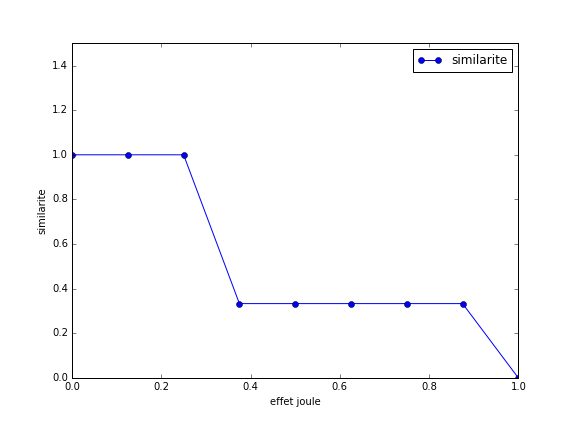
\includegraphics[scale=0.50]{courbe_similarite_selon_EJ_pour_epsilon_075.png}
\caption{ Le coefficient de similarit\'e en fonction des pertes par {\em effets joules} pour $epsilon=0.75$.}
\label {courbeEJCoef}
\end{figure}
\begin{figure}
\centering
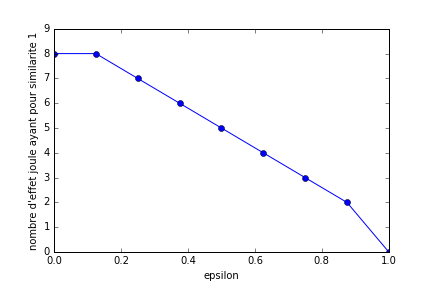
\includegraphics[scale=0.65]{courbe_epsilon_selon_nbreEJ_pour_similarite_1.png}
\caption{ R\'elation inverse entre $\epsilon$ et $EJ$: $8$ en ordonn\'e correspond \`a $[0,1]$, $7$ \`a $[0, 0.875]$ }
\label {courbeEpsilonEJ}
\end{figure}

% conclusion
Ces deux exp\'eriences montrent que la d\'ecision de l'ORACLE  a une r\'elation inverse avec les pertes par effets joules ($EJ$). En effet, plus $\epsilon$ est petit plus les pertes par effets joules sont grandes et plus les d\'ecisions de l'ORACLE sont erron\'ees.
\begin{equation}
	\epsilon > 1 - EJ
\end{equation}

\subsubsection{Complexit\'e de l'algorithme de couverture}
La complexit\'e de l'algorithme est au pire en $O(m \times \Delta(G_M))$ avec $m$ le nombre d'ar\^etes et $\Delta(G_M)$ le degr\'e maximum du graphe.
On rappelle que l'algorithme de Lehot \cite{decompositionEnCliques} a une complexit\'e en $O(m) +E$. 
Le facteur $\Delta(G_M)$ dans notre algorithme, du \`a la recherche de la d\'ecomposition en deux cliques $C_1$ et $C_2$ est n\'ecessaire \`a la determination de l'ensemble des sommets $v$ tels que $Cliq(v) = -1$, en nombre le plus petit possible.
\newline

En conclusion, si le graphe $G_M$ est bien un line-graphe, l'algorithme  de couverture trouvera une d\'ecomposition du voisinage d'un sommet en une ou deux cliques de fa\c con unique (voir les lemmes pr\'ec\'edents). 
Une fois ce sommet supprim\'e, le graphe restant est toujours un line-graphe, et la propri\'et\'e se propage.
Donc, si $G_M$ est un line graphe, cet algorithme en trouvera toujours la couverture de corr\'elation unique.
% ------------> a debuger l'algo et a l'ecrire
	\subsection{Algorithme de correction}
		We consider the initial graph $G$ with vertices $v$ such that this neighborhood does not form a clique i.e $cliq(v) = -1$. 
We suggest an algorithm which modify the initial set $E_C$ by adding or deleting edges in order to get a {\em linegraph}. 
%Given that labeled vertices $v$ to $cliq(v) = -1$ in a given order $z_1 , z_2 , ..., z_t$. 
Given that vertices $v$ are labeled to $cliq(v) = -1$ in a given order $z_1 , z_2 , ..., z_t$. 
Let $E_C^i$ be the edge set of $G$ after the (i-1)-th vertices had been already treated in that order.  
In the following chapter, we denote by  $z = z_i$  a vertex and by ${\cal C}^{i}$ the set of cliques of $G_C$ at the i-th step. Thus $E_C^1 = E_C$ et ${\cal C} = {\cal C}^{1}$.

Let  $C(z) = \{C_1 , . . . , C_k \}$ be a set of all cliques from ${\cal C}^{i}$ of size at least 3 which  $z$ belongs to. 
We notice that the intersection of each pair of cliques from $C(z)$ gives the vertex $z$. 
We define by $S(z)$ the union of a set of all adjacent vertices $v$ of $z$ in the cliques $K_2 = \{v, z\} \in {\cal C}^i$ of size $2$ and a set of all adjacent vertices $v$ of $z$ such that $[v, z]$ is not covered by any clique of ${\cal C}^i$. 

\begin{equation}	
S(z) = \{ v \in \Gamma_{G}(z) | \{z,v\} \in C^i \} \cup \{ v \in \Gamma_{G}(z) | \{z,v\} \notin E(c), \forall c \in {\cal C}^i\}
\end{equation} 
with $E(c)$, an edge set of clique $c$.

\begin{definition}
Two cliques $C$ and $C'$ from ${\cal C}(z)$ are  {\bf contractables} if any edge $[u,v]$  of $E_C^i$ such that $u \in C$ and $v \in C'$ is not covered  by a clique (other that $\{u,v\}$) in ${\cal C}$. 
\end{definition}


\begin{definition}
A clique $C \in {\cal C}^i$ is {\bf neighbour} of $z$ if $C \notin {\cal C}(z)$ and $card(C \cap S(z)) \ge 2$.
The dependency of a clique $C$ neighbour of $z$ is the set $D_{z}(C) \subset {\cal C}(z)$ such as $C' \in D_{z}(C) $ and $C' \cap C \cap \Gamma_{G}(z) \ne \emptyset$.
A clique $C$ is {\bf increasing} if and only if it is neighbour of $z$ and $D_{z}(C)$ is contractable or empty.
\begin{equation}
voisine(z) = \{C \in {\cal C}^i \mbox{ } | \mbox{ } C \notin C(z) \mbox{ } \& \mbox{ } card(C \cap S(z)) \ge 2 \} \newline
\end{equation}
\begin{equation}
D_{z}(C) = \{ C' \in C(z) \mbox{ }|  \mbox{ } C' \cap C \cap \Gamma_{G}(z) \ne \emptyset \}
\end{equation}

\end{definition}

We denote by an \textbf{increasement} of $z$, an union of 
a vertex $\{z\}$, 
an increasing clique $C$ of $z$ and 
a contraction of cliques of $D_{z}(C)$.

\begin{definition}
We denote by a {\bf compression} de $z$, a triplet $T$ represented by $\pi_1$, $\pi_2$, $\pi_s$  defined by: 
	
\begin{itemize}	
	\item  $\pi_1$ (resp. $\pi_2$) can be one of two forms:
	\begin{enumerate} 		
		\item $\pi_1$ (respectively $\pi_2$) is the union of $\{z\}$, a subset $C_1$ (resp. $C_2$) of cliques from  ${\cal C}(z)$ such as any pair $C$ and $C'$ of $C_1$ (resp. $C_2$) is contractable and a subset $S_1$ (resp. $S_2$) of vertices $v \in S(z)$ not belonging to any clique such as:			
$$ \forall v \in S_1,~\forall x \in C_1, \not\exists C' \in {\cal C}~t.q.~card(C')>2~~et~~\{v,x\} \subset C'$$			
		\item $\pi_1$ (resp. $\pi_2$)  is an increasement of $z$.
	\end{enumerate}
	\item  $\pi_1$ and $\pi_2$ can not be simultaneously reduce to $\{z\}$ and  $\pi_1 \cap \pi_2 = \{z\}$.
	\item $\pi_S=\Gamma_G(z)-~((\pi_1 \cap \Gamma_G(z)) \cup(\pi_2 \cap \Gamma_G(z)))$ such as edge set $\{[z,v]\in E_{C}^{i}:~v\in \pi_S\}$  is not disconnecting. 	
	\item the triplet $\pi_{1} \cap \Gamma_{G}(z)$, $\pi_{2} \cap \Gamma_{G}(z)$, $\pi_{S} \cap \Gamma_{G}(z)$ is a 3-partition of $\Gamma_{G}(z)$.
\end{itemize}

\end{definition}


Such a compression always consists for example in whether 
$\pi_1 = \{z\} \cup C_i \in C(z)$, 
$\pi_2 =  \emptyset$,
$\pi_s = \gamma_G(z) -(\gamma_G(z) \cup C_i) $  if ${\cal C}(z)$ is not empty.
Else, 
$\pi_1 = \{z\} \cup \{ v \in \gamma_G(z)  \} $, 
$\pi_2 =  \emptyset$,
$\pi_s = \gamma_G(z) - \{v\} $
is an another compression.
Another example compression is given in the figure \ref{correctionGraph}.
\begin{centering} 
\begin{figure}[htb!]
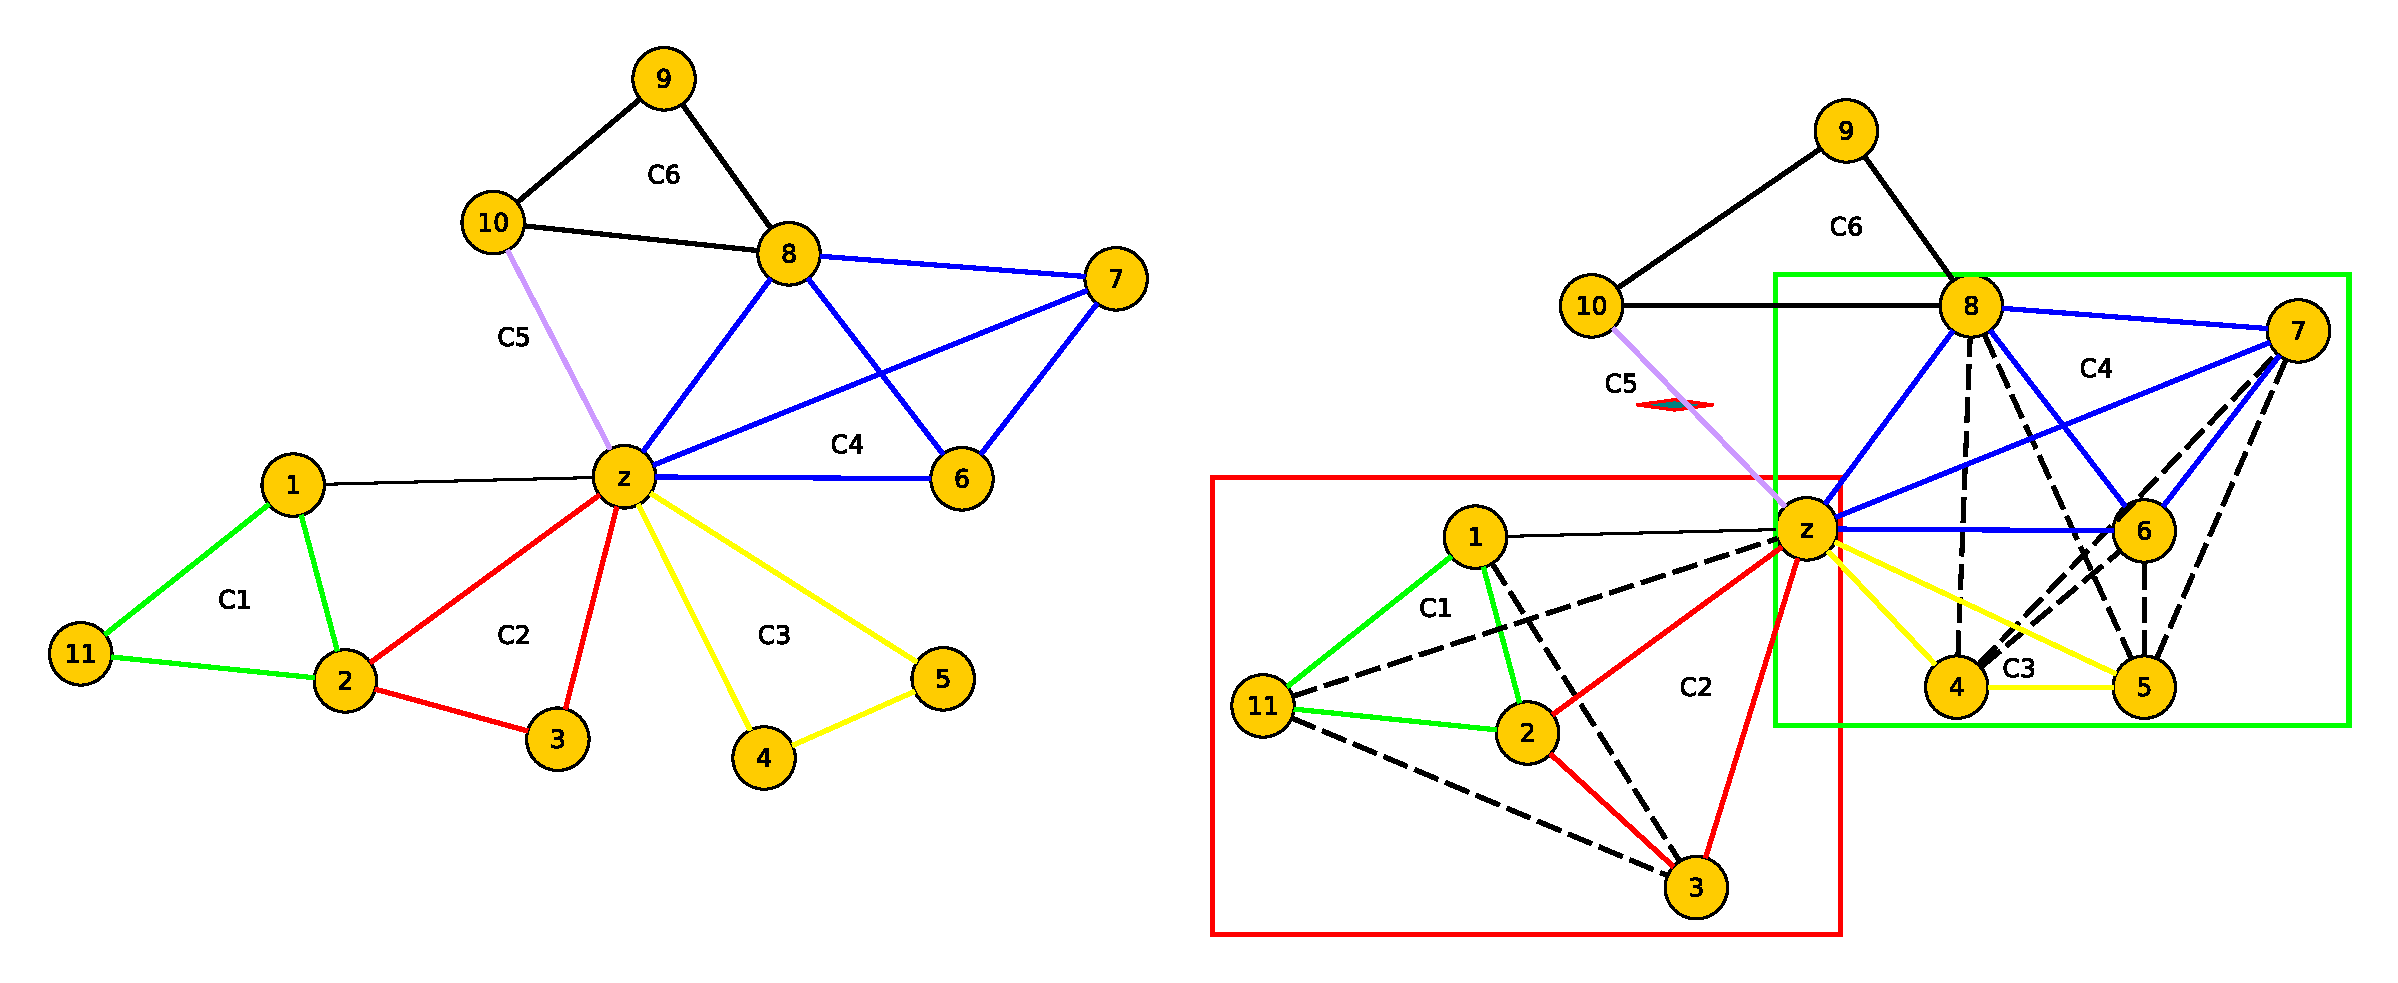
\includegraphics[scale=0.30]{./imagesLineGraphes/correctionGraph.eps} \vspace{-0.5em}
\caption{an compression example}
\label{correctionGraph}
\end{figure}
\end{centering} 


The $\pi_{1},\pi_{2},\pi_{S}$ compression cost is defined by:
$$c(T) = | \{\{u,v\} \in \pi_{1}:~[u,v]\not\in E_{C}^{i}\}| + |\{\{u,v\} \in \pi_2:~[u,v]\not\in E_{C}^{i}\}| +~ |\pi_S| $$



%Let $Cost(z)$ the minimum compression cost of $v$.
Let $Cost(z)$ be the minimum cost of a correlation cover of $v$. 

Our goal is to modify $G_C$ such as $z$ will be covered by one or two cliques from $\pi_1$ and $\pi_2$.
To do this, the cost of this change $ c(T) $ takes into account the edges to add (linked to $\pi_1$ and $\pi_2$) and to remove (linked to $\pi_S$).


Thus, {\bf applying a compression} $T=\pi_1,\pi_2,\pi_s$ consists in adding in $E_0$ the edges defined by the sets $\{\{u,v\} \in \pi_1:~[u,v]\not\in E_{C}^{i}\}$ (would be covered by the clique $\pi_1$) and $\{\{u,v\} \in \pi_2:~[u,v]\not\in  E_{C}^{i}\}$ (would be covered by the clique $\pi_2$), and to delete the edges $\{[z,v] \in  E_{C}^{i}:~v\in \pi_S\}$. 
From then on, vertex $z$ belongs to two cliques $\pi_1$ et $\pi_2$. 
We realize the following updates to obtain ${\cal C}^{i+1}$ and $E_{C}^{i+1}$ :

\begin{itemize} 
	\item delete all cliques ${\cal C}_z$ covered by $\pi_1$ in  ${\cal C}^{i}$.
	\item delete all cliques of cardinal $2$ covered by  $\pi_1$ and  $\pi_2$ in ${\cal C}^{i}$,        
	\item add $\pi_1$ and $\pi_2$ in ${\cal C}^{i}$, delete from $E^{i}_C$ all edges $\{[z,v] \in E_C^{i}:~v\in \pi_S\}$. 
	\item assign $Cliq(z)$ to $1$ (if $\pi_1$ or $\pi_2$ is empty) or $2$ (else).
\end{itemize}

This procedure has the following properties:
\begin{property}
We consider a compression operation.
Let ${\cal C}^{i+1}$ the set obtained from ${\cal C}^{i}$ after a compression.
\begin{enumerate}
\item each edge of $G_{C}$ covered by one or two cliques in ${\cal C}^{i}$ remains in ${\cal C}^{i+1}$.
\item each edge covered by only one clique in ${\cal C}^{i}$ and not deleted in ${\cal C}^{i}$  remains in ${\cal C}^{i+1}$.
\item the vertex $z$ is covered by one or two cliques in ${\cal C}^{i+1}$ (the number of vertices covered increases by $1$ compared to the number in ${\cal C}^{i}$).
\end{enumerate}
\end{property}

Thus, for each vertex $z_i$ of list $z_1, z_2, \ldots, z_t$ taken in that order, we consider a minimum compression cost $c_{m}^{i}$ and we apply it.
The property above ensure at the end of process, we obtain a correlation graph $G_{C}^{t} = (V, E_{C}^{t})$ whose the modified set $\cal C$ is a correlation cover.
The line-distance verifies $DL( G_{C}^{0}, G_{C}^{t}) \le \sum_{1 \le i \le t } c_{m}^{i}$.
We notice that during a $j > 1$ step, the vertex $z_{j}$ and its neighborhood is covered by one or two cliques after the processing of $j-1$ previous vertices. If no compression is applied to it, we have an identity compression and thus $c_{m}^{i} = 0$.

\subsection{Global algorithm behavior} 
In complexity, the two algorithms process once each vertex in the graph.
 The complexity of vertex processing is exponential depending of each vertex degree and the cliques to which the vertex belongs, here again depends on the size and the number of cliques. 
Global algorithm is thus {\bf pseudo-polynomial} depending on the degree  of the graph. 
Given the initial graph, an algorithm running  is a way to select vertices in the {\bf covered algorithm} and then the order to take labeled vertices $z$ such as $cliq(z) = -1$ in the correction algorithm.

	\subsection{Complexit\'e des algorithmes}
		%\documentclass[onecolumn, 12pt]{book}
%
%\usepackage[latin1]{inputenc}   
%\usepackage{amsmath}
%\usepackage{algorithm}
%\usepackage{algorithmic} 
%%\usepackage[T1]{fontenc}
%
%%\usepackage[francais]{babel}     
%\usepackage{layout}    
%\usepackage[top=2cm, bottom=2cm, left=2cm, right=2cm]{geometry} 
%\usepackage{setspace}
%\usepackage{soul}
%\usepackage{color} 
%\usepackage{verbatim}
%\usepackage{moreverb}
%\usepackage{listings}
%\usepackage{url}
%\usepackage{graphicx}
%\usepackage{epstopdf}
%\usepackage{caption}
%\usepackage{setspace}
% \usepackage{amssymb} % used for not exists symbol ==> \nexists
% 
%\title{complexite des algorithmes}
%\author{Wilfried Ehounou}
%\date{\oldstylenums{\today}} 
%
%\newtheorem{definition}{D\'efinition}
%\newtheorem{property}{Propri\'et\'e}
%\newtheorem{theorem}{Theorem}
%\newtheorem{claim}[theorem]{Claim}
%\newtheorem{proposition}[theorem]{Proposition}
%\newtheorem{lemma}[theorem]{Lemma}
%\newtheorem{corollary}[theorem]{Corollary}
%\newtheorem{conjecture}[theorem]{Conjecture}
%\newtheorem{observation}{Observation}
%\newtheorem{example}{Exemple}
%\newtheorem{remark}{Remark}
%
%%---insert paragraph (use 4) and subparagraph (use 5) to table of contents
%\setcounter{tocdepth}{4} 
%\setcounter{secnumdepth}{4}
%
%%---- path figures ----
%\graphicspath{{/home/willy/Documents/courbePython/courbeDegreCoutMinAleatoire_11_09_2017/}
%{/home/willy/Documents/courbePython/courbeDegreCoutMinAleatoire_11_10_2017/}
%{/home/willy/Documents/courbePython/courbeDegreCoutMinAleatoire_11_09_2017/comparaison_MethodesCorrection_fctDeCout_permut_aleatoire_coutMin_degreMin/}{/home/willy/Documents/latexDoc/redactionThese/chap3_linegraphs/imagesLineGraphes/}}
% 
%\begin{document}
%\maketitle
%\tableofcontents

%\section{Comportement des algorithmes de couverture et de correction}
L'algorithme de correction traite au plus une fois chaque sommet du graphe.
La complexit\'e de traitement de chaque sommet est exponentiel en fonction du degr\'e de chaque sommet et des cliques auxquelles il appartient, la encore en fonction  de son degr\'e en taille et en nombre.
L'algorithme global (couverture et correction) est donc pseudo-polynomial en fonction du degr\'e du graphe.
\newline

Nous mettons une conjecture sur le comportement de l'algorithme.
Etant donn\'e un graphe de d\'epart, une ex\'ecution de l'algorithme est un ordre dans lequel seront trait\'es les sommets dans l'algorithme de couverture, puis un ordre dans lequel seront pris les sommets $z \in sommets\_1$.
\newline
Consid\'erons un graphe de corr\'elation $G$ n'\'etant pas isomorphe \`a un graphe de la figure \ref{graphe2Couverture}. On dira que $G$ est non-ambigu.

Deux ar\^etes $[u,v]$ et $[u',v']$ de $G$ seront dit {\bf clique-independantes} si et seulement si il n'existe pas de cliques $C$ dans la line couverture  de $G$ telle que 
$C \cap \{u,v\} \cap \{u',v'\} \ne \emptyset$

\begin{conjecture}
Si $G'=(V, E')$ est un graphe obtenu en supprimant un ensemble d'ar\^etes deux \`a deux clique-independantes d'un graphe de corr\'elation non-ambigu $G=(V,E)$, alors il existe une ex\'ecution de l'algorithme qui transforme $G'$ en G
\end{conjecture}

%\end{document}

%--------------------------------------------------------------------
%------- 		graphe root		---------------------
%--------------------------------------------------------------------
\section{D\'etermination de la topologie du r\'eseau \'energ\'etique}
	% ----
% decouverte de topologie du reseau energetique
% ----
Soient $\cal C$, l'ensemble des cliques de la line graphe $G_C$ et $G$ le graphe racine de $G_C$. \newline
Chaque clique $C_k \in {\cal C}$ correspond \`a un sommet du graphe racine $G$. \newline 
Soit $u = \{``ENTRANT'', ``SORTANT'', ``NONE''\}$, l'ensemble des marquages de chaque ar\^ete tel que les \'etiquettes $``ENTRANT''$ et $``SORTANT''$ sont associ\'ees respectivement \`a l'ar\^ete $a_i$ entrante et sortante du sommet $C_k$.
\newline
%-- definition de S_1 e S_2
Soient $S_1$ et $S_2$ l'ensemble des arcs entrants et sortantes du sommet $C_k$.
\begin{equation}
S_\alpha = \{ S_{\alpha,i}, \hspace{0.2 em} \forall i \le 2^{card(C_k)+1}  \}
\end{equation}
avec $i$, le nombre de sous-ensemble de $C_k$ et $\alpha = \{1,2\}$. Le sous-ensemble $S_{\alpha,i}$ peut \^etre  l'ensemble vide $\emptyset$.
 
 %--  ORACLE
 \begin{definition}
 Soit la clique $C_k$ de la couverture {\cal C}.
 Un couple $(S_1,S_2)$ de sous-ensembles de $C_k$ est {\bf valide} si 
 \begin{itemize}
 \item $S_1 \ne S_2$
 \item $S_1 \cup S_2 = C_k$
 \item $S_1 \cap S_2 = \emptyset$
 \end{itemize}
 \end{definition}
 
 \begin{definition}
 Soit une fonction binaire $ORACLE$ d\'efinit de $S_1 \times S_2 \rightarrow \{0,1\}$, avec le couple valide $(S_1,S_2)$.
 La fonction $ORACLE$ renvoie $1$ si et seulement si la loi de conservation autour du sommet $C_k \in G$ est respect\'ee c'est-\`a-dire : 
 \begin{equation}
 \forall a_i \in S_1, \forall a_j \in S_2, \sum_{a_i \in S_1} gp(a_i) - \sum_{a_j \in S_2} gp(a_j) \le \epsilon
 \end{equation}
 avec $\epsilon$ les pertes par effets joules, $gp(a_i)$ le flot dans l'arc $a_i \in E(G)$.
 \end{definition}
 
 \begin{property}
 Si $ORACLE(S_1, S_2) = 1$ alors l'ensemble  $S_1$ est l'ensemble des arcs entrants et  $S_2$ l'ensemble des arcs sortants du sommet $C_k \in G$.
 \end{property} 
Les arcs de $S_1$ et $S_2$ ne concourent pas \`a un sommet $C_k$ lorsque  $ORACLE(S_1, S_2) = 0$.

\begin{theorem}
\label{arcsentrantsSortants}
%Un arc $a_i$ est soit {\em entrant}, soit {\em sortant} mais jamais les deux.
Si un sommet $a_i \in G_C$ appartient \`a deux cliques $C_{k_1}, C_{k_2} \in {\cal C}$ alors 
l'arc  $a_i \in E(G)$ est soit entrant de $C_{k_1}$  et sortant de $C_{k_2}$ ou soit entrant de $C_{k_2}$  et sortant de $C_{k_1}$.
\end{theorem}

\begin{proof}
D'apr\`es la d\'efinition \ref{line-couverture}, le sommet $a_i$ appartient \`a deux cliques $C_{k_1}$ et $C_{k_2}$ au maximum. 
Cela implique qu'il existe une ar\^ete entre les sommets $C_{k_1}$ et $C_{k_2}$ dans $G$.
Soient $S_1, S_2 \subset C_{k_1}$ et $S_1, S_2 \subset C_{k_2}$ telles que $ORACLE(S_1, S_2) = 1$ et $ORACLE(S_3, S_4) = 1$.
Comme  $S_1 \cap S_2 = \emptyset$, $S_3 \cap S_4 = \emptyset$ et aussi  $C_{k_1} \cap C_{k_2} = \{a_i\}$, on a quatre choix possibles :
$a_i \in S_1 \cap S_3$, $a_i \in S_1 \cap S_4$, $a_i \in S_2 \cap S_3$, $a_i \in S_2 \cap S_4$.
\newline
Si $a_i$ est entrant et sortant \`a $C_{k_1}$ et $C_{k_2}$ alors $a_i \in S_1 \cap S_3$ ou  $a_i \in S_2 \cap S_4$. 
On en d\'eduit qu'il existe une boucle sur le sommet $C_{k_1}$ et $C_{k_2}$. 
Cela est impossible parce que $G$ est un $DAG$. 
\newline
Alors $a_i$ est entrant \`a $C_{k_1}$ $=>$ $a_i \in S_2 \cap S_3$ ou  $a_i$ sortant \`a $C_{k_2}$  $a_i \in S_1 \cap S_4$. 
\end{proof}

Soit $A$ l'ensemble des cliques $C_j$ tel que $card(C_j) = min\{ card(C_k), C_k \in {\cal C}\}$.
\newline
Soit la fonction $f$ d\'efinie sur $ V(G_C) \times A \rightarrow \{0,1\}$ retournant $1$ si le sommet $a_i^u$ ne poss\`ede aucune \'etiquette c'est-\`a-dire labellis\'e \`a $None$.
$$ f(a_i^u, C_j) = \begin{cases} 1 \hspace{0.2 em} si \hspace{0.2 em} M(a_i^u, C_j) \ne None \\ 0 \hspace{0.2 em} sinon \end{cases}$$
La fonction $MA$ calcule le nombre de sommets labellis\'e dans une clique $C_k$.
$$MA(C_k) =  \sum_{a_i^u \in C_k} f(a_i^u,C_k) $$
Soient la clique $C_m$ telle que  $MA(C_m) = max\{ MA(C_j), C_j \in A\}$ et $B$ l'ensemble des sommets de la clique $C_m$ tel que $M(C_m, a_j^v) == None, \forall a_j^v \in B$. 


%nommer l'algorithme
\begin{algorithm}
\caption{Decouverte\_graphe\_racine}
\noindent DEBUT\\
\noindent 1. Initialisation des \'etiquettes des sommets $a_i$ de $G_C$, et $C_k \in {\cal C}$ \\
\noindent $M( C_k, a_i^u) = None$ \\
~2. \indent {\bf Tant que} il existe une  ar\^ete de $G_C$ ($E(G_C)$) \\
	\indent~~~~~~{\bf Faire}\\
%~3.		\indent~~~~~~~~ $f(a_i^u, C_k) = \{ 1 si M(a_i^u, C_k) \ne None, 0 sinon$\\
%~3.		\indent~~~~~~~~ $MA(C_k) = \sum_{a_i^u \in C_k} f(a_i^u,C_k) $\\
%~3.	       	\indent~~~~~~~~choisir $a_i^u, C_k$ tel que $min\{ \hspace{0.1em} d(a_i^u),  a_i^u \in C_k \}$ et $max\{ M(C_k, a_i^u) \neq None \hspace{0.2em}, \forall a_i^u \in C_k \}$ \\
%~3.	       	\indent~~~~~  choisir $a_i^u, C_k$ tel que $min\{ \hspace{0.2em} card(C_k),  C_k \in {\cal C} \}$ et $max\{ MA(C_k) , \forall C_k \in {\cal C} \}$ et $M(C_k,a_i^u) == None$ \\
~3.		\indent~~~~~~~~choisir $A = \{C_j , card(C_j) = min\{ card(C_k), C_k \in {\cal C} \}\}$ \\
~4.		\indent~~~~~~~~choisir $C_k$ tel que $MA(C_k) = max\{ MA(C_j), C_j \in A\} $ \\
%~5.		\indent~~~~~~~~choisir $a_i^u$ al\'eatoirement dans $B = \{a_j^v , M(C_k, a_j^v) == None \hspace{0.2em} \forall a_j^v \in C_k\}$ \\
~5.       	\indent~~~~~~~~{\bf Si} il existe $S_1$ et $S_2$ tel que $S_1 \cup S_2 = \emptyset $ et $S_1 \cup S_2 = C_k $ et $ORACLE(S_1, S_2, M )= 1 $ \\
~6.	       	\indent~~~~~~~~~~~~{\bf alors}\\
~7.	       	\indent~~~~~~~~~~~~ $S_1^k = sommets\_marques(S_1, M)(^1)$; \\
~8.	       	\indent~~~~~~~~~~~~ $S_2^k = sommets\_marques(S_2, M)$; \\
~9.		\indent ~~~~~~~~~~~~{\bf Pour tout} $a_i^K \in S_1 - S_1^k$ {\bf Faire} \\
~10.		\indent ~~~~~~~~~~~~~ $M(C_k, a_i^K) = ``ENTRANT''$ \\
~11.		\indent ~~~~~~~~~~ {\bf Pour tout} $a_i^K \in S_2 - S_2^k$ {\bf Faire} \\
~12.		\indent ~~~~~~~~~~~~~ $M(C_k, a_i^K) = ``SORTANT''$ \\
~13.		\indent~~~~~~~~~~ $E(G_{C}) =  E(G_C)  - E(G_C[C_k])$ \\
~14.		\indent~~~~~~~~~~ ${\cal C} =  {\cal C}  - C_k$ \\
~15.       	\indent~~~~~~~~{\bf FinSi} \\
~16. \indent {\bf FinTant que} \\
~17. \indent {\bf Pour tout} $a_i^u \in V(G_C)$ {\bf Faire} \\
~18. \indent ~~~ $C_1, C_2$ = $Couverture\_Cliques(a_i^u, M)(^2)$\\
% C_1 != emptyset et C_2 != \emptyset
~19. \indent ~~~ {\bf Si } $C_1 \neq \emptyset$ et $C_2 \neq \emptyset$ {\bf Alors} \\
~20. \indent ~~~~~~  {\bf Si}  $M(C_1, a_i^u) == ``SORTANT''$ {\bf Alors} \\
~21. \indent ~~~~~~~~~~~~ $Mat(C_1)$ += $C_2$ $(^3)$ \\  
~22. \indent ~~~~~~  {\bf Fin Si} \\
~23. \indent ~~~~~~  {\bf Si}  $M(C_2, a_i^u) == ``SORTANT''$ {\bf Alors} \\
~24. \indent ~~~~~~~~~~~~ $Mat(C_2)$ += $C_1$ $(^3)$ \\  
~25. \indent ~~~~~~  {\bf Fin Si} \\
~26. \indent ~~~ {\bf Fin si} \\
% C_1 != emptyset et C_2 = \emptyset
~27. \indent ~~~ {\bf Si } $C_1 \neq \emptyset$ et $C_2 == \emptyset$ {\bf Alors} \\
%~29. \indent ~~~~~~  {\bf Si}  $M(C_1, a_i^u) == ``SORTIE''$ {\bf Alors} \\
%~30. \indent ~~~~~~~~~~~~ $Mat(C_1)$ += $EXT\_SORTIE\_C1$ $(^3)$\\  
%~31. \indent ~~~~~~  {\bf Fin Si} \\
~28. \indent ~~~~~~  {\bf Si}  $M(C_1, a_i^u) == ``ENTRANT''$ {\bf Alors} \\
~29. \indent ~~~~~~~~~~~~ $Mat(EXT\_a_i^u)$ += $C1$ $(^3)$\\  
~30. \indent ~~~~~~  {\bf Fin Si} \\
~31. \indent ~~~~~~  {\bf Si}  $M(C_1, a_i^u) == ``SORTANT''$ {\bf Alors} \\
~32. \indent ~~~~~~~~~~~~ $Mat(C_1)$ += $EXT\_a_i^u$ $(^3)$ \\  
~33. \indent ~~~~~~  {\bf Fin Si} \\
~34. \indent ~~~ {\bf Fin si} \\
~35. \indent {\bf Fin Pour} \\
~36. \noindent {\bf Return} Mat\\
% C_1 = emptyset et C_2 != emptyset
%~36. \indent ~~~ {\bf Si } $C_1 == \emptyset$ et $C_2 \neq \emptyset$ {\bf Alors} \\
%~37. \indent ~~~~~~  {\bf Si}  $M(C_2, a_i^u) == ``SORTIE''$ {\bf Alors} \\
%~38. \indent ~~~~~~~~~~~~ $Mat(C_2)$ += $EXT\_SORTIE\_C2$ $(^3)$ \\  
%~39. \indent ~~~~~~  {\bf Fin Si} \\
%~40. \indent ~~~~~~  {\bf Si}  $M(C_2, a_i^u) == ``ENTREE''$ {\bf Alors} \\
%~41. \indent ~~~~~~~~~~~~ $Mat(C_2)$ += $EXT\_ENTREE\_C2$ $(^3)$\\  
%~42. \indent ~~~~~~  {\bf Fin Si} \\
%~43. \indent ~~~ {\bf Fin si} \\
\noindent FIN\\
\end{algorithm}

$^1$ : Cette fonction retourne les sommets de l'ensemble $S_1$ ou $S_2$ labellis\'es \`a $``ENTREE''$ ou $``SORTANT''$. Initialement, Ces sommets sont \'etiquett\'es \`a $``None''$.

$^2$ : Cette fonction renvoie les cliques couvrantes une ar\^ete $a_i^u$ avec $C_1 \ne \emptyset$. Si $a_i^u$ est couvert par une clique alors $C_2 = \emptyset$.

$^3$ : $EXT\_a_i^u$ est un sommet du graphe racine $G$.
\newline

L'algorithme {\em Decouverte\_graphe\_racine} d\'ebute par l'initialisation des sommets de $G_C$ \`a $''None''$.
Tant qu'il existe une ar\^ete dans notre line graphe $G_C$, on choisit la plus petite clique $C_k$ dont le maximum de sommets de cette clique est labellis\'e soit par $''ENTRANT''$ ou soit par $''SORTANT''$ (lignes $3-4$).
On partitionne la clique $C_k$  en deux sous-ensembles valides $S_1$ et $S_2$ tels que $S_1$ et $S_2$ correspondent, respectivement, \`a l'ensemble des arcs entrants et sortants du graphe racine $G$.
Les sommets labellis\'es de $S_1$ not\'es $S_1^k$ portent l'\'etiquette $''ENTRANT''$ tandis que ceux labellis\'es en $''SORTANT''$ sont not\'es $S_2^k$ (lignes $6-12$). 
Ensuite nous mettons \`a jour l'ensemble des ar\^etes et la line-couverture de $G_C$ (lignes $13-14$). 
\newline
Une fois termin\'e l'orientation des ar\^etes de $G$ qui  sont les sommets labellis\'es du line graphe $G_C$ (lignes $2-16$), nous construisons la liste d'adjacence de chaque sommet de $G$ (lignes $17-36$).
Nous recherchons la couverture d'un sommet $a_i^u$ de $G_C$.
\newline 
Si le sommet  $a_i^u$ est couvert par une seule clique alors $C_2 = \emptyset$. Dans ce cas, cela signifie qu'il existe un arc entre le sommet $C_1$ et le sommet $EXT\_a_i^u$ que nous avons cr\'ee. Cet arc a pour extr\'emit\'e initiale $C_1$ si $a_i^u$ est labellis\'e par $''SORTANT''$ sinon pour extr\'emit\'e initiale $EXT\_a_i^u$ si $a_i^u$ est labellis\'e par $''ENTRANT''$ (lignes $27-34$).
\newline
Dans le cas o\`u le sommet $a_i^u$ est couvert par deux cliques non vides $C_1, C_2$, nous ajoutons un arc entre ces deux cliques.
D'apr\'es le th\'eor\`eme  \ref{arcsentrantsSortants} stipulant qu'un sommet de $G_C$ est $''ENTRANT''$ de $C_1$ et $''SORTANT''$ de $C_2$ et vice-versa, nous d\'efinissons  $C_1$ comme extr\'emit\'e initiale de cet arc si $a_i^u$ est labellis\'e par $SORTANT$ dans cette clique $C_1$ sinon $C_2$ si $a_i^u$ est labellis\'e par $SORTANT$ dans cette clique $C_2$ (lignes $19-26$).

\subsection{Complexit\'e de l'algorithme {\em Decouverte\_graphe\_racine} }

La fonction $Couverture\_Cliques$ a une complexit\'e constante $O(1)$ alors que la complexit\'e de la  fonction $sommets\_marques$ depend du nombre de sommets dans $S_1$. Dans le pire des cas, sa complexit\'e est $O(n)$ avec $n = E(G)$ le nombre  d'arcs de $G$. Donc les lignes $17-35$ s'ex\'ecutent en $O(n)$ dans le pire des cas. 
\newline
Consid\'erons une line-couverture ${\cal C}$  de taille $K$,  une clique $C_i \in {\cal C}$ de taille $p_i$ et $k_i$ le nombre de sommets marqu\'es dans $C_i$. 
\newline
Le nombre de couples valides $(S_1,S_2)$ pour la clique $C_i$ avec $k_i$ sommets marqu\'es est $2^{p_i -k_i}$. 
Au traitement de la premi\`ere clique de ${\cal C}$ de taille minimale $C_1$, il existe $0$ sommets marqu\'es. Le co\^ut $R_{cv_1}$ de couples valides est $R_{cv_1} = 2^{p_1}$.
Au traitement de la seconde clique $C_2$, il existe $k_2 \ge 0$ et son co\^ut est  $R_{cv_2} = 2^{p_2 - k_2}$.
Il existe une clique $C_\alpha$ \`a partir de laquelle $k_\alpha > 0, \alpha \le K$.
On remarque que $p_\alpha - k_\alpha$ est d\'ecroissant car $k_\alpha$ augmente apr\`es chaque traitement de cliques. 
Cela signifie qu'\`a la selection de la derni\`ere clique $C_k$, son co\^ut  est de $R_{cv_K} = 1$. 
Le co\^ut est decroissant \`a chaque traitement c'est-\`a-dire 
$$2^{p_{\alpha} - k_{\alpha}} \ge 2^{p_{\alpha+1} - k_{\alpha+1}} \ge \cdots \ge 2^{p_K - k_K}$$ 
Le co\^ut des couples valides de ${\cal C}$ est 
$$R_{cv} = O(2^\gamma), \gamma = max\{card(C_i), \forall C_i  \in \{C_1, \cdots, C_\alpha\} \}$$
car il depend de la clique $C_i \in \{C_1, \cdots, C_\alpha\} \subset {\cal C}$.
\newline
Le co\^ut des lignes $3-4$ depend de $p_i$ et $K$ ($O(p_i) + O(K)$) et celui des lignes $7-14$ est de $O(p_i^2)$.
\newline
Soit le co\^ut $R$ de la boucle  {\em Tant que}. Il est de 
$$ R = O(p_i) + O(K) + O(p_i^2) + O(2^\gamma) \simeq O(2^\gamma)$$

La complexit\'e de {\em Decouverte\_graphe\_racine} est {\em pseudo-exponentielle} car l'exposant $\gamma$ est la taille d'une clique de taille interm\'ediaire.

%Consid\'erons les instructions dans le boucle {\em Tant que}, $K$ le cardinal de ${\cal C}$ et $p$ le cardinal de la clique de taille minimale de ${\cal C}$ c'est-\`a-dire $card(A) = p$. 
%\newline
%$R_i$ est le co\^ut de la boucle {\em Tant que} au traitement de la $i^eme$ clique de $G_C$ et $C\_oracle$ le co\^ut de la fonction $ORACLE$.
%S\'electionnons le premier clique de $G_C$. Son co\^ut est :
%$$R_1 = p \times C_oracle(S_{1p}, S_{2p}) $$.
%Le co\^ut  du deuxi\`eme sommet est :
%$$R_2 = p \times C_oracle(S_{1p}, S_{2p})  + (p-1) \times C_oracle(S_{1p-1}, S_{2p-1})  $$.
%Le co\^ut des $n$ sommets de $G_C$ est :
%$$R_K = \sum_{k = 0}^{K-1} (p-k) \times C_oracle(S_{1p-k}, S_{2p-k})$$
%
%La particularit\'e de l'ORACLE est que pour $k \ge p$, tous les sommets de la clique $C_k$ sont labellis\'es entrainant qu'on ne genere aucuns sous-ensembles de $C_k$. Cela implique que  $C_oracle(S_{1p-k}, S_{2p-k}) = 1$. \newline
%Cela revient \`a dire que le co\^ut $R_K$ est d\'ecroissant en fonction de $K$. \newline
%G\'en\'erer tous  sous-ensembles de $C_k$ de taille $p$ est une combinaison de 
%$card(P(E)) = 2^{p}$ et toutes les paires de $P(E)$ vaut au pire des cas $\frac{2^p * (2^p - 1)}{2}$. 
%Alors  le  cout  $C_oracle(S_{1p}, S_{2p}$ est $O(2^p)$ ===> FAUX
%%%%% A discuter avec SERGES ---> trouver le nombre de tuples provenant des sous ensembles  de C_k de taille $p$
%Donc le co\^ut de $R_K$ est  
%$$R_K = p \times O(2^p) + (p-1) \times O(2^{(p-1)}) + \cdots + 1 \times O(2^0)$$
%$$ R_K $$
%PAS FINI



		
%--------------------------------------------------------------------
%------- 	graphes iourtes		 ---------------------
%--------------------------------------------------------------------
\section{Correction particuli\`ere de Graphes : Graphes Iourtes }
%	

On se doit de consid\'erer le cas o\`u dans le graphe de corr\'elation initial $G_C$, il existe des sommets $z$ tels que $Cliq(z) = -1$ et qu'aucun tel sommet $z$ n'est contenu dans une clique et qu'aucun de ses voisins n'est contenu par une clique.
Ce qui implique que tout sommet du graphe est dans la situation de $z$.

\begin{lemma}
Pour tout entier $n \ge 12$, il existe un graphe $G$ d'au moins $n$ sommets dans lequel aucun sommet n'est couvert par une ou deux cliques.
\end{lemma}

\begin{proof}
Ce lemme est tout d'abord bas\'e sur le fait que le graphe $G_0$ de la figure \ref{graphe_iourte_G0} le v\'erifie.
On obtient, \`a partir de $G_0$, un graphe avec $3$ sommets suppl\'ementaires v\'erifiant toujours cette propri\'et\'e en r\'ealisant la modification suivante. 
Ce graphe $G$ distingue trois sommets A, B, C. 
On remplace chaque ar\^ete $[A,B]$, $[B,C]$, $[A,C]$ par une chaine de longueur $2$.
Les sommets ainsi cr\'ees deviennent les nouveaux sommets distingu\'es A, B, C que l'on relie par un cycle de longueur $3$.
On peut ainsi propager cette modification autant de fois que n\'ecessaire pour atteindre $n$.
Ce qui cl\^ot la preuve du lemme.
\end{proof}

\begin{centering} \vspace{-0.5em}
\begin{figure}[htb!] \vspace{-0.5em}
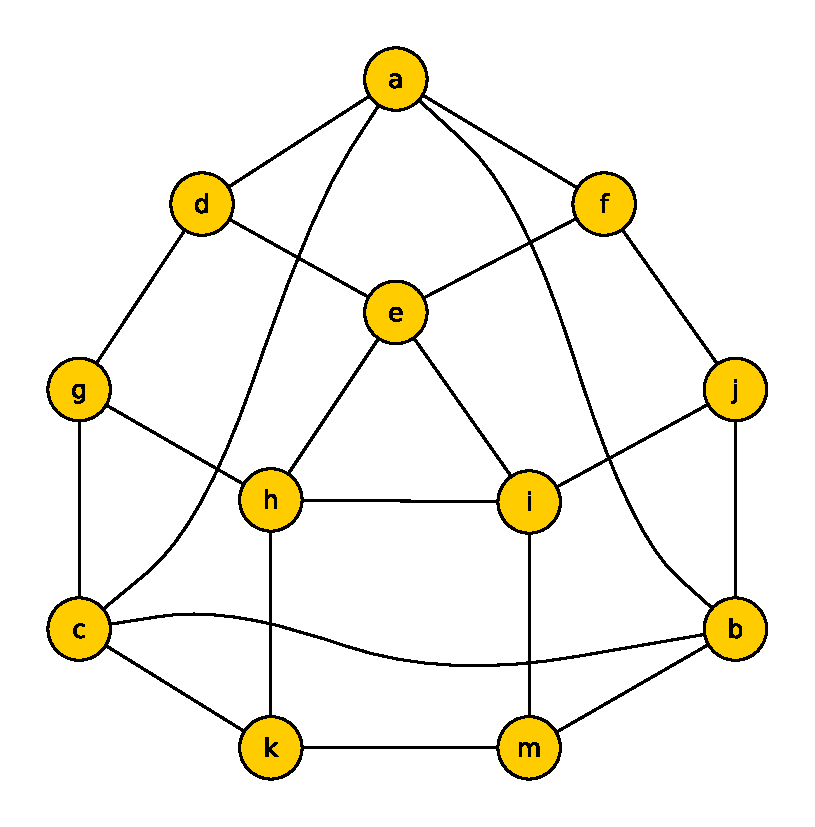
\includegraphics[scale=0.75]{grapheIourteG0.eps}
\caption{ Graphes $G_0$ o\`u aucun sommet n'est couvert par aucune clique }
\label{graphe_iourte_G0} 
\end{figure}
\end{centering} 

Notons $G_0^k$ avec $k \ge 1$ le graphe obtenu \`a partir de $k$ op\'erations de propagation \`a partir de $G_0$, graphe contenant donc $3k+12$ sommets, $6k+21$ ar\^etes et de degr\'e maximum \'egal \`a $4$.

\begin{theorem}
La distance-line de $G_0^k$ v\'erifie
$$ DL(G_0^k) \le 3k+6 $$
\end{theorem}

\begin{proof}
La figure \ref{graphe_iourte_G0_une_execution} d\'ecrit un line graphe $LG_0$ couvrant $G_0$ avec $6$ ar\^etes ne figurant pas dans $G_0$.
Le line graphe $LG_0^k$ couvrant et \`a distance $3k+6$ de $G_0^k$ est obtenu \`a partir  de $LG_0^{k-1}$ en supprimant une ar\^ete sur deux dans le cycle de taille $6$ form\'e par les anciens sommets $A$, $B$ et $C$ de $G_0^{k-1}$ et les nouveaux sommets $A$, $B$ et $C$ de $G_0^{k}$ (c'est-\`a-dire la suppression de $3$ ar\^etes).
Chaque ar\^ete restante sur ce cycle forme une nouvelle clique de taille $2$ et le nouveau cycle de taille $3$ entre $A$, $B$ et $C$  forme une nouvelle clique de taille $3$ (qui remplace la pr\'ec\'edente dans $LG_0^{k-1}$)....
\end{proof}

\begin{centering} \vspace{-0.5em}
\begin{figure}[htb!] \vspace{-0.5em}
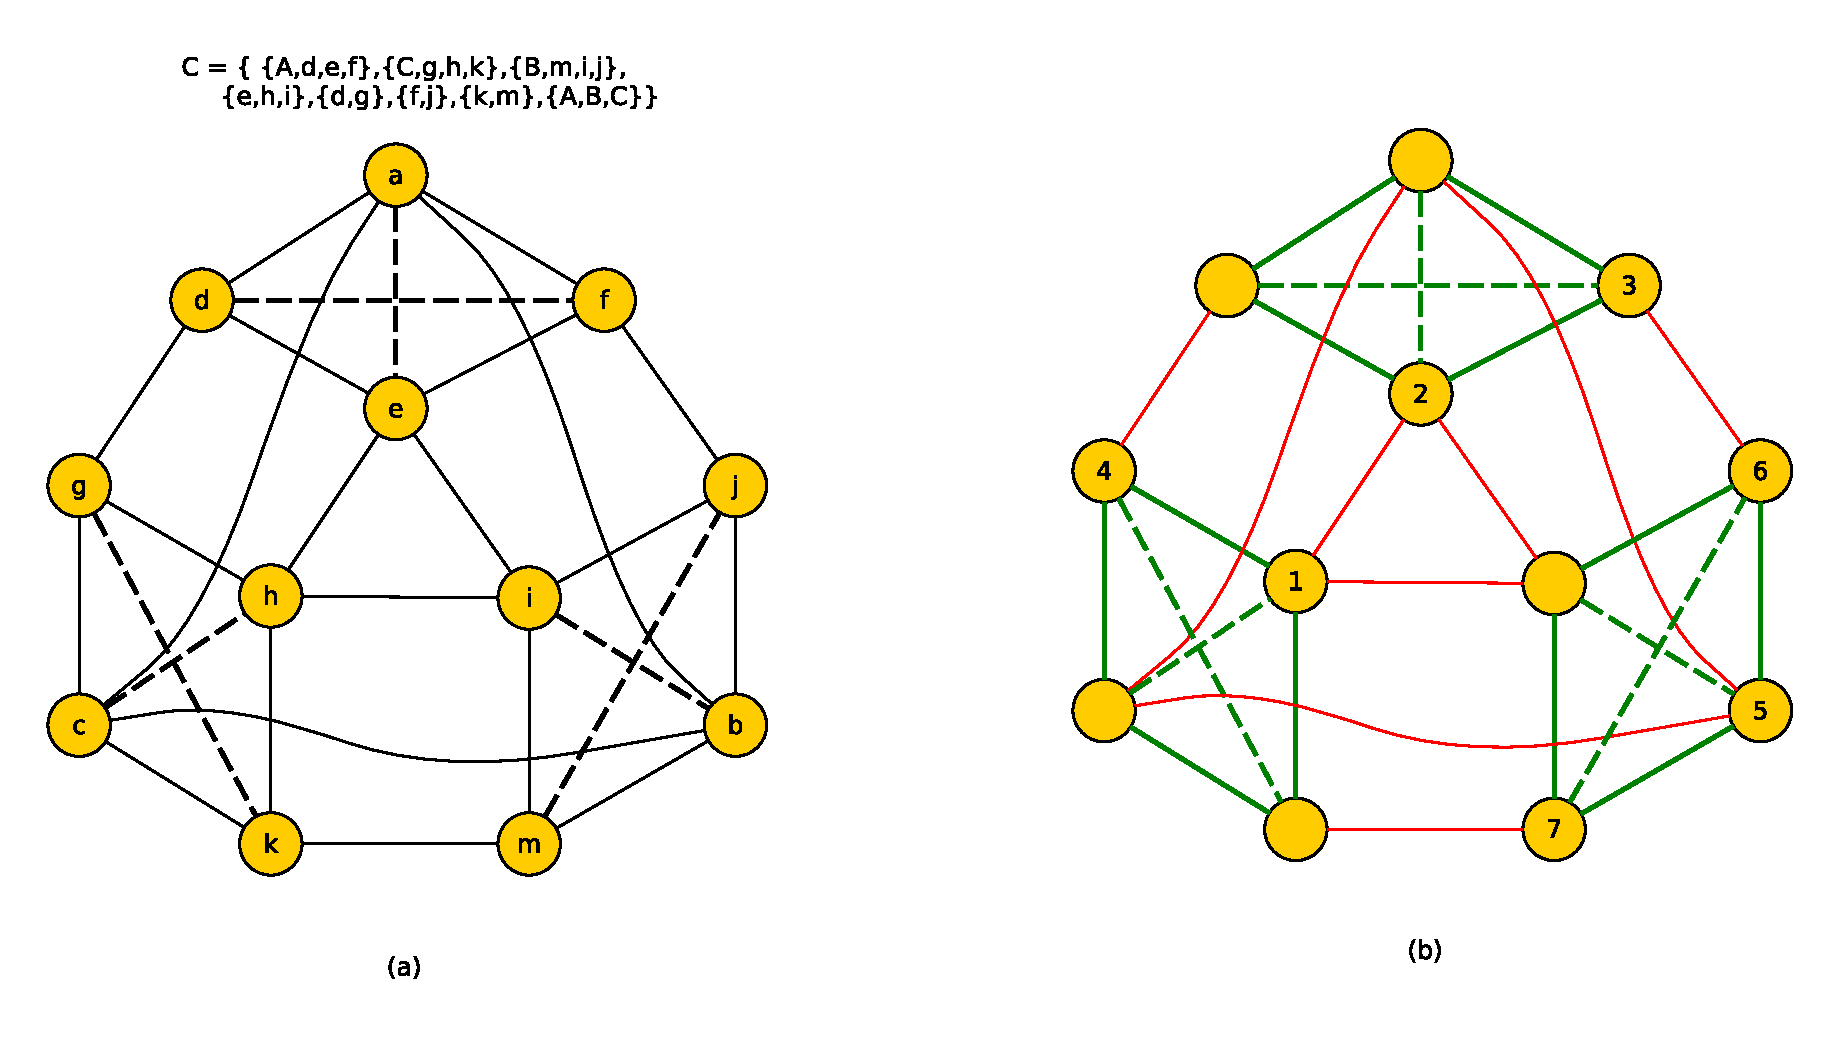
\includegraphics[scale=0.57]{grapheIourteG01eExecution.eps}
\caption{ (a) line graphe $LG_0$ \`a distance de Hamming $6$ de $G_0$ avec une couverture par cliques maximales $C$, et (b) une ex\'ecution (parmi celles possibles) de l'algorithme de compression transformant $G_0$ en $LG_0$}
\label{graphe_iourte_G0_une_execution} 
\end{figure}
\end{centering} 


 

\end{document}